\documentclass[11pt, a4paper]{article}

\usepackage[utf8]{inputenc}
\usepackage[T1]{fontenc}
\usepackage{geometry}
\geometry{top=2.5cm, bottom=2.5cm, left=2.5cm, right=2.5cm}
\usepackage{amsmath}
\usepackage{amssymb}
\usepackage{hyperref}
\usepackage{enumitem}
\usepackage{booktabs}
\usepackage{multirow}
\usepackage{graphicx}
\usepackage{caption}
\usepackage{subcaption}
\usepackage{rotating}
\usepackage{float}

\begin{document}

\section*{Report: Machine Learning Pipeline for Drug-Target Interaction (DTI)}

\section*{Introduction}
In this report, we construct an interpretable machine learning pipeline that systematically dissects the binding affinity into discrete
topological heuristics and continuous physicochemical fields. By conducting a rigorous feature ablation study—progressing from pure topological
memorization (Morgan fingerprints) to a strictly continuous, orthogonal basis of 2D/3D quantum and thermodynamic fields—we aim to quantify
exactly how much of the binding variance can be explained by fundamental laws of physics versus local substructure matching.

\subsection*{1. Feature Engineering: Translating Chemistry into CS Concepts}
Predicting the binding affinity ($pK_i$) between a ligand and a protein is fundamentally a problem of modeling intermolecular forces. To make this
tractable for machine learning, we map the textual representation of a molecule (SMILES) into continuous and discrete vector spaces. The features
are grouped by their level of abstraction: from simple heuristics to 3D continuous fields.

\subsubsection*{1.1. The Baselines: Heuristics and Macroscopic Thermodynamics}
This group acts as a strong global prior for the model, describing the bulk properties of the molecule and its general "drug-likeness."
\begin{itemize}[leftmargin=*]
    \item \textbf{Lipinski's Rule of 5 Violations}: A well-known pharmacological heuristic. It counts how many of four fundamental thresholds
    (MW, LogP, HBD, HBA) a molecule violates. In ML terms, this is a highly predictive aggregated discrete feature that separates biologically
    viable ligands from random chemical noise.
    \item \textbf{LogP (Partition Coefficient)}: Represents the lipophilicity of the molecule. In the context of the \textit{hydrophobic effect},
    water forms a highly ordered structural network. When a lipophilic ligand enters a protein pocket, water is displaced, causing a massive
    increase in system entropy. LogP is the primary weight defining the "energy reward" the system gets simply by moving the ligand out of
    the aqueous solvent.
    \item \textbf{Molecular Weight (MW)}: Represents the spatial bulk of the molecule. Acts as a strict boundary condition: a molecule that is
    too large simply cannot satisfy the geometric constraints of a target cavity.
    \item \textbf{H-Bond Donors (HBD) \& Acceptors (HBA)}: Integer counts of specific atoms (like Oxygen and Nitrogen) capable of forming
    hydrogen bonds. These are the strict "lock-and-key" conditional nodes; without matching H-bond pairs in the protein, optimal binding cannot occur.
    \item \textbf{TPSA (Topological Polar Surface Area)}: Estimates the surface area over all polar atoms. It serves as a penalty term:
    high TPSA means the molecule strongly interacts with water, requiring a high energetic cost to "strip" this water away before binding to
    the protein.
\end{itemize}

\subsubsection*{1.2. 2D Graph Topology and Spectral Invariants}
Here, the molecule is treated as an undirected graph $G=(V,E)$, where nodes are atoms and edges are bonds.
\begin{itemize}[leftmargin=*]
    \item \textbf{Morgan Fingerprints (Radius 2, 1024-bit)}: Conceptually identical to the Weisfeiler-Lehman graph hashing algorithm. It iteratively
    hashes the neighborhood of each node up to a depth of 2 edges, folding the result into a fixed-length binary vector. It acts as a Bag-of-Words
    for chemical subgraphs (pharmacophores), identifying if specific "plug shapes" exist in the ligand.
    \item \textbf{Wiener Index}: A topological invariant defined as the sum of the shortest-path distances between all pairs of nodes in the graph.
    It encodes the overall structural branching and compactness of the molecule into a single scalar.
    \item \textbf{Laplacian Spectrum ($\lambda_{max}, \lambda_{fiedler}$)}: Extracted from the graph Laplacian $L = D - A$.
    \begin{itemize}
        \item \textit{Fiedler Value ($\lambda_2$)}: The algebraic connectivity of the graph. From a thermodynamic perspective, a highly connected,
        rigid graph (high $\lambda_2$) has fewer degrees of freedom. When it binds to a protein, it loses less conformational entropy compared
        to a highly flexible chain. This spectral feature mathematically proxies the $-T\Delta S$ penalty in the Gibbs free energy equation.
        \item \textit{Spectral Radius ($\lambda_{max}$)}: Captures the maximum degree of bipartite partitioning in the graph, offering an additional
        metric for graph complexity.
    \end{itemize}
\end{itemize}

\subsubsection*{1.3. 3D Spatial Geometry}
Features derived from generating the lowest-energy 3D conformation of the graph.
\begin{itemize}[leftmargin=*]
    \item \textbf{SASA (Solvent Accessible Surface Area)}: The continuous 3D counterpart to TPSA. It computes the actual geometric surface area
    that a rolling water molecule can touch, providing a high-fidelity continuous feature for the desolvation penalty.
    \item \textbf{Normalized Principal Moments of Inertia (NPR1, NPR2)}: The 3D point cloud of atoms is analyzed via its inertia tensor.
    The eigenvalues are normalized to classify the overall geometric shape into a 2D continuous phase space bounded by three extremes:
    perfectly spherical, flat (disk-like), or elongated (rod-like). This helps the model learn steric compatibility with different types of
    protein pockets (e.g., narrow tunnels vs. flat surface grooves).
\end{itemize}

\subsubsection*{1.4. Continuous Quantum and Electrostatic Fields}
To capture the long-range forces driving the interaction, we compute node-level and graph-level physical fields.
\begin{itemize}[leftmargin=*]
    \item \textbf{Gasteiger Charge Span ($\Delta Q$)}: The difference between the maximum and minimum partial charges computed via iterative
    electronegativity equalization. It acts as a proxy for the dipole moment, giving the model a scalar representation of long-range electrostatic
    pull.
    \item \textbf{Extended H\"uckel Theory (EHT) Energies}:
    \begin{itemize}
        \item \textit{Fermi Energy ($E_F$)}: The energy of the highest occupied molecular orbital (HOMO). A continuous feature defining how
        "eager" the molecule is to share electrons (its reactivity) with the target protein.
        \item \textit{Total Electronic Energy}: Defines the baseline thermodynamic stability of the specific 3D embedding used.
    \end{itemize}
    \item \textbf{Coulomb Matrix Spectrum ($C_{max}, C_{trace}$)}: The Coulomb matrix encodes the N-body electrostatic repulsion between all atoms,
    where off-diagonal elements are $Z_i Z_j / R_{ij}$ ($Z$ being atomic numbers, $R$ being Euclidean distance). Because raw matrices are sensitive
    to the arbitrary ordering of nodes (atoms), we extract the maximum eigenvalue and the trace. These are \textit{permutation-invariant}
    representations of the molecule's global 3D electrostatic distribution, making them robust features for gradient boosting or SVR models.
\end{itemize}

\subsection*{2. ETL and Orchestration Pipeline}

The system architecture isolates data sanitization from model training to prevent data leakage and noise propagation.

\subsubsection*{2.1. Signal Isolation (ETL)}

Biological datasets are inherently noisy. The \texttt{DataLoader} and \texttt{DataCleaner} modules enforce strict data integrity:
\begin{itemize}[leftmargin=*]
    \item \textbf{Sub-graph Pruning (Desalting)}: Raw SMILES often contain disconnected components (e.g., counter-ions or salts). A stripping
    algorithm is applied to retain only the largest continuous sub-graph (the active ingredient).
    \item \textbf{Label Noise Filtering}: If the dataset contains multiple binding affinity measurements for the same SMILES, they are aggregated
    by the median. Crucially, if the standard deviation of these conflicting measurements exceeds a predefined threshold, the sample is entirely
    dropped to prevent the model from fitting to ambiguous ground truth labels.
\end{itemize}

After cleaning, the dataset contains 2442 unique SMILES with high-confidence $pK_i$ values, ready for feature extraction.

Before defining the feature space and training the estimators, it is critical to understand the thermodynamic landscape of the curated dataset.
Figure \ref{fig:target_dist} illustrates the distribution of the target variable, the binding affinity ($pK_i$). 

Notably, the target exhibits a distinct \textit{bimodal distribution} (a mixture of two Gaussians). The smaller left peak ($pK_i \approx 6.2$)
typically represents primary screening "hits" with micromolar affinity, while the dominant right peak ($pK_i \approx 7.8$) corresponds to highly
optimized "leads" and established drugs with nanomolar affinity.
\begin{figure}[H]
    \centering
    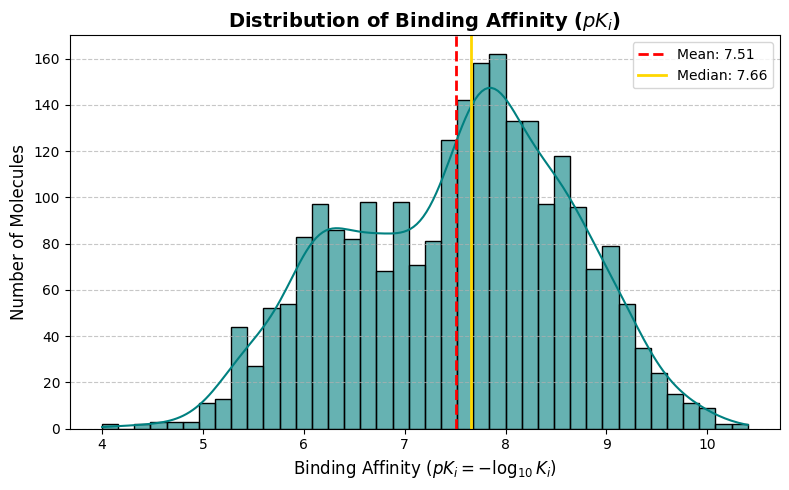
\includegraphics[width=0.7\textwidth]{figures/data_distribution.png}
    \caption{\textbf{Distribution of Binding Affinity ($pK_i$):} The dataset demonstrates a bimodal thermodynamic distribution. The presence of both early-stage weak binders (left shoulder) and highly optimized potent inhibitors (main peak) provides a robust, multi-order magnitude gradient for training regression algorithms.}
    \label{fig:target_dist}
\end{figure}

\subsubsection*{2.2. Dynamic Orchestration}
The \texttt{ExperimentRunner} handles the continuous integration of features and model validation:
\begin{itemize}[leftmargin=*]
    \item \textbf{Lazy Evaluation \& Caching}: The \texttt{FeatureBuilder} utilizes a central registry to compute only the features explicitly
    requested. Expensive computations (like 3D ETKDG embedding) are cached per molecule, drastically reducing pipeline execution time.
    \item \textbf{Robust Evaluation}: The final continuous target ($pK_i$) is evaluated using K-Fold Cross-Validation. Performance is tracked
    using $R^2$ (variance explained) and Mean Absolute Error ($MAE$), which provides a highly interpretable error metric in logarithmic
    concentration units directly applicable to drug discovery.
\end{itemize}

\subsubsection*{2.3. Feature Selection and Orthogonalization}
To ensure the stability of the tree-based estimators and to derive meaningful feature importances, we implemented an automated correlation
filter to establish an orthogonal physicochemical basis. Continuous features exhibiting a Pearson correlation coefficient $|r| > 0.85$ were
analyzed for physical redundancy. 

Crucially, the decision of which feature to discard from a collinear pair is not arbitrary. Whenever a highly correlated pair of descriptors
is detected, the pipeline evaluates their individual predictive utility by computing their \textbf{Mutual Information (MI)} with the target
variable ($pK_i$). Unlike simple correlation, mutual information quantifies the actual reduction in uncertainty about the binding affinity
provided by a given feature, capturing both linear and non-linear thermodynamic dependencies. The algorithm systematically drops the feature
with the lower MI score, ensuring that the retained basis is maximally informative.

\section*{3. Experimental Results and Discussion}

To rigorously evaluate the predictive power of our physicochemical descriptors and to understand the decision boundaries of different ML estimators,
we conducted a systematic feature ablation study.

\subsection*{3.1. Experimental Design}
We defined four distinct feature spaces (Experiments A through D) to isolate the impact of topological heuristics versus continuous
quantum/thermodynamic fields:
\begin{itemize}[leftmargin=*]
    \item \textbf{Experiment A (Baseline - Topology Only)}: 1024-bit Morgan Fingerprints. Tests the capacity of the models to predict binding
    affinity purely by recognizing local substructures (pharmacophores).
    \item \textbf{Experiment B (Macro-Prior)}: Morgan Fingerprints + Macroscopic Thermodynamics (MW, LogP, TPSA, HBD, HBA). Tests if global
    constraints improve the topological baseline.
    \item \textbf{Experiment C (2D Spectral Physics)}: Morgan + Macro + 2D Graph Physics ($\Delta Q$, Laplacian Spectra). Evaluates whether
    mathematically cheap 2D continuous fields and entropy proxies can enhance predictions without the need for expensive 3D embedding.
    \item \textbf{Experiment D (Full 3D Physicochemical Space)}: All features combined (Morgan + Macro + 2D + 3D EHT \& Coulomb Matrices).
    Determines if the computationally heavy 3D quantum mechanics and spatial electrostatics provide a statistically significant breakthrough in
    model accuracy.
    \item \textbf{Experiment E (Pure Physics \& Thermodynamics)}: Strictly continuous physical fields (Macro + 2D + 3D) \textit{without}
    Morgan Fingerprints. This tests whether $\approx 20$ fundamental physical descriptors can match the predictive power of a highly sparse
    1024-dimensional topological vector.
\end{itemize}

\subsection*{3.2. Quantitative Performance}
Table \ref{tab:results} presents the K-Fold cross-validation metrics for four different regression architectures:
Random Forest (RF), CatBoost, LightGBM (LGBM), XGBoost and Support Vector Regression (SVR). 

\newpage
\begin{sidewaystable}[htbp]
\centering
\caption{Predictive Performance ($pK_i$) across different Feature Spaces and ML Architectures. Results are presented as $Mean \pm Std$ from 5-Fold Cross-Validation.}
\label{tab:results}
\vspace{0.3cm}
\resizebox{\textwidth}{!}{%
\begin{tabular}{@{}llccccc@{}}
\toprule
\textbf{Feature Space} & \textbf{Metric} & \textbf{RF} & \textbf{CatBoost} & \textbf{LGBM} & \textbf{XGBoost} & \textbf{SVR} \\ \midrule

\multirow{3}{*}{\textbf{Exp A: Morgan Only}} 
 & $R^2$          & $0.7161 \pm 0.0298$ & $0.6960 \pm 0.0228$ & $0.7034 \pm 0.0279$ & $0.7219 \pm 0.0305$ & $0.7407 \pm 0.0258$ \\
 & $RMSE$         & $0.5914 \pm 0.0327$ & $0.6125 \pm 0.0262$ & $0.6047 \pm 0.0306$ & $0.5854 \pm 0.0348$ & $0.5653 \pm 0.0302$ \\
 & $MAE$          & $0.4274 \pm 0.0226$ & $0.4477 \pm 0.0139$ & $0.4392 \pm 0.0163$ & $0.4174 \pm 0.0229$ & $0.4032 \pm 0.0235$ \\ \midrule

\multirow{3}{*}{\textbf{Exp B: Morgan + Macro}} 
 & $R^2$          & $0.7156 \pm 0.0290$ & $0.7022 \pm 0.0200$ & $0.7046 \pm 0.0252$ & $0.7292 \pm 0.0268$ & $0.7449 \pm 0.0249$ \\
 & $RMSE$         & $0.5920 \pm 0.0305$ & $0.6063 \pm 0.0244$ & $0.6037 \pm 0.0285$ & $0.5778 \pm 0.0316$ & $0.5608 \pm 0.0298$ \\
 & $MAE$          & $0.4266 \pm 0.0184$ & $0.4432 \pm 0.0128$ & $0.4347 \pm 0.0174$ & $0.4098 \pm 0.0216$ & $0.3983 \pm 0.0233$ \\ \midrule

\multirow{3}{*}{\textbf{Exp C: Morgan + Macro + 2D}} 
 & $R^2$          & $0.7147 \pm 0.0233$ & $0.7058 \pm 0.0218$ & $0.7147 \pm 0.0234$ & $0.7328 \pm 0.0234$ & $0.7447 \pm 0.0253$ \\
 & $RMSE$         & $0.5932 \pm 0.0257$ & $0.6025 \pm 0.0244$ & $0.5932 \pm 0.0261$ & $0.5741 \pm 0.0292$ & $0.5609 \pm 0.0294$ \\
 & $MAE$          & $0.4269 \pm 0.0187$ & $0.4388 \pm 0.0139$ & $0.4267 \pm 0.0170$ & $0.4085 \pm 0.0196$ & $0.3990 \pm 0.0239$ \\ \midrule

 \multirow{3}{*}{\textbf{Exp D: Morgan + Macro + 2D + 3D}} 
 & $R^2$          & $0.7100 \pm 0.0238$ & $0.7036 \pm 0.0192$ & $0.7120 \pm 0.0214$ & $0.7266 \pm 0.0227$ & $0.7472 \pm 0.0236$ \\
 & $RMSE$         & $0.5980 \pm 0.0269$ & $0.6049 \pm 0.0224$ & $0.5961 \pm 0.0247$ & $0.5807 \pm 0.0275$ & $0.5582 \pm 0.0269$ \\
 & $MAE$          & $0.4312 \pm 0.0195$ & $0.4406 \pm 0.0120$ & $0.4268 \pm 0.0151$ & $0.4115 \pm 0.0200$ & $0.3980 \pm 0.0216$ \\ \midrule

\multirow{3}{*}{\textbf{Exp E: Pure Physics}} 
 & $R^2$          & $0.5793 \pm 0.0241$ & $0.5819 \pm 0.0274$ & $0.5938 \pm 0.0275$ & $0.6099 \pm 0.0190$ & $0.5067 \pm 0.0315$ \\
 & $RMSE$         & $0.7208 \pm 0.0273$ & $0.7187 \pm 0.0333$ & $0.7082 \pm 0.0302$ & $0.6942 \pm 0.0232$ & $0.7804 \pm 0.0301$ \\
 & $MAE$          & $0.5272 \pm 0.0169$ & $0.5358 \pm 0.0214$ & $0.5217 \pm 0.0192$ & $0.5097 \pm 0.0137$ & $0.5753 \pm 0.0209$ \\ \bottomrule
\end{tabular}%
}
\end{sidewaystable}

\subsection*{3.3. Dimensionality Reduction in Physical Spaces (Exp C, D \& E)}
As we introduced continuous physical fields, the automated orthogonalization pipeline aggressively pruned redundant features to combat
multicollinearity (see Figure \ref{fig:corr_matrices}).
In Experiment C, Molecular Weight (\texttt{mw}) was dropped due to extreme collinearity with the Wiener Index. In the 3D spaces
(Experiments D and E), the extensive properties that fundamentally scale with the molecule's size—such as Molecular Weight (MW),
Wiener Index (topological node count), and Coulomb Trace (sum of nuclear charges)—exhibit extreme multicollinearity with Solvent Accessible
Surface Area (SASA). Because the exact 3D SASA provides a higher-fidelity representation of the desolvation penalty and steric footprint,
it naturally yields a higher mutual information score with $\Delta G$ and is algorithmically retained over its cheaper 1D proxies. Additionally,
collinear shape constraints (e.g., NPR1 being strictly bounded by NPR2) are pruned based on their target MI scores to maintain a linearly
independent and maximally predictive feature space.


\begin{figure}[htbp]
    \centering
    \begin{subfigure}[b]{0.48\textwidth}
        \centering
        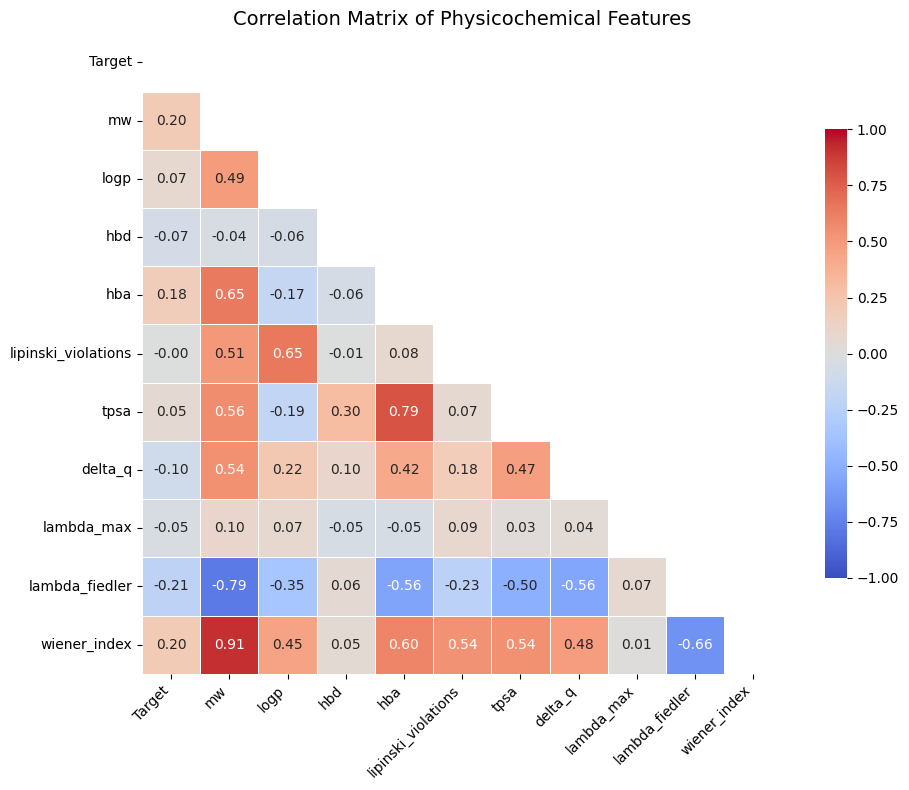
\includegraphics[width=\textwidth]{figures/corr_matrix_c.png}
        \caption{Experiment C: 2D Physics Space}
    \end{subfigure}
    \hfill
    \begin{subfigure}[b]{0.48\textwidth}
        \centering
        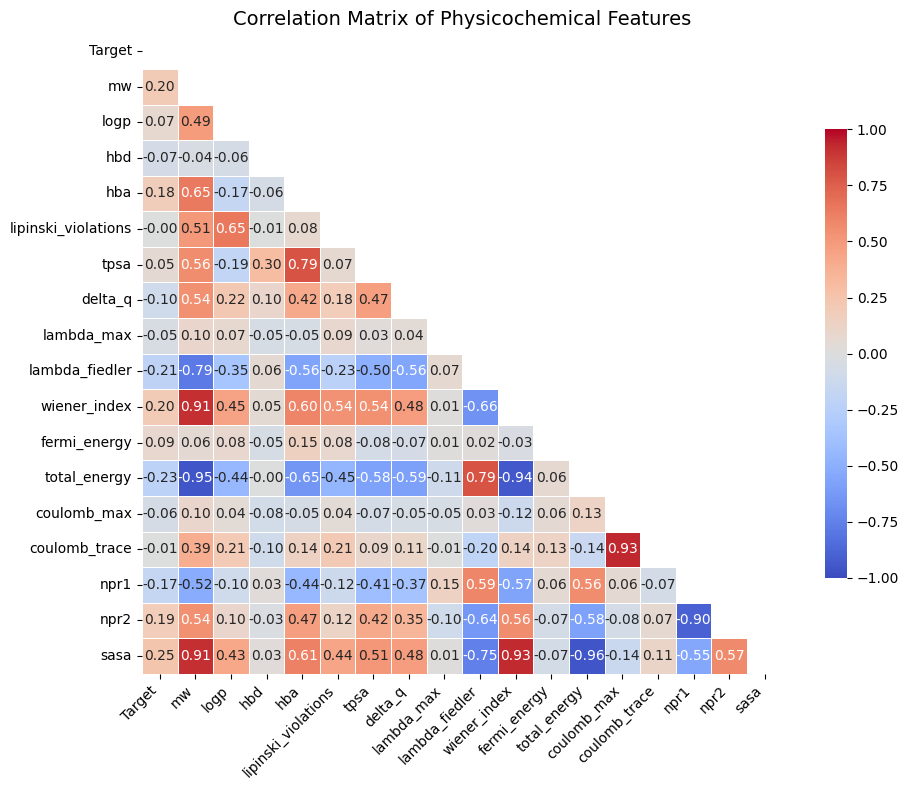
\includegraphics[width=\textwidth]{figures/corr_matrix_d.png}
        \caption{Experiments D \& E: 3D Physics Space}
    \end{subfigure}
    \caption{\textbf{Orthogonalization Process:} Pearson correlation matrices used to detect multicollinearity. Highly collinear pairs
    ($|r| > 0.85$), such as Molecular Weight vs. Wiener Index, were systematically pruned to retain the most descriptive, linearly independent
    physical features.}
    \label{fig:corr_matrices}
\end{figure}

\newpage
\subsection*{3.4. Interpretability and Feature Contributions}

To extract actual physical insights from our tree-based models, we utilized SHapley Additive exPlanations (SHAP).
Figures \ref{fig:expA_grid}-\ref{fig:expE_grid} displays Feature Importances and SHAP values for Experiments A-E.

\begin{figure}[p]
    \centering
    % ROW 1: Random Forest
    \begin{subfigure}[b]{0.48\textwidth}
        \centering
        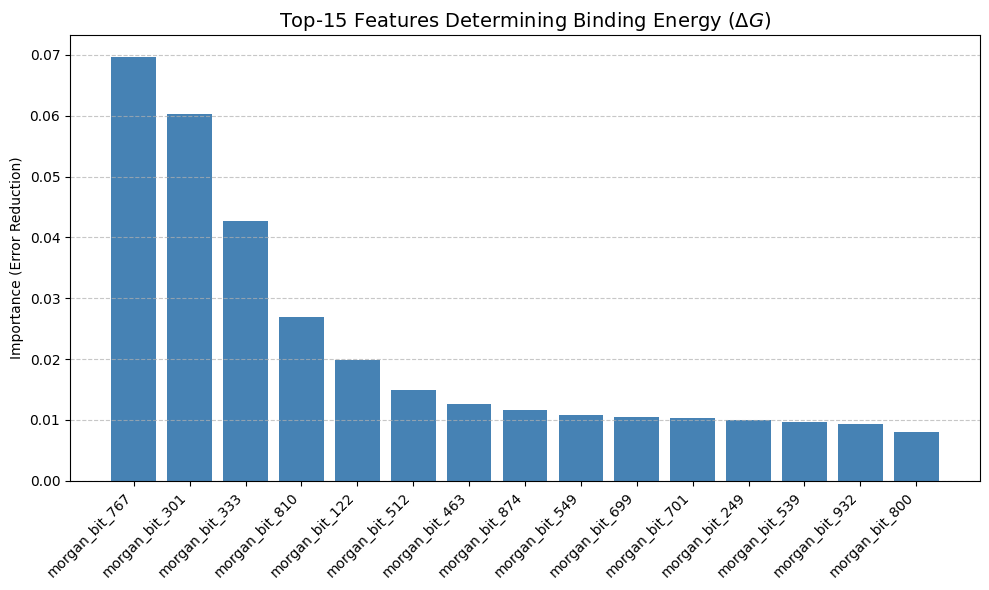
\includegraphics[width=\textwidth, height=0.2\textheight, keepaspectratio]{figures/rf_a_imp.png} % Replace with RF Importance
        \caption{RF: Feature Importance}
    \end{subfigure}
    \hfill
    \begin{subfigure}[b]{0.48\textwidth}
        \centering
        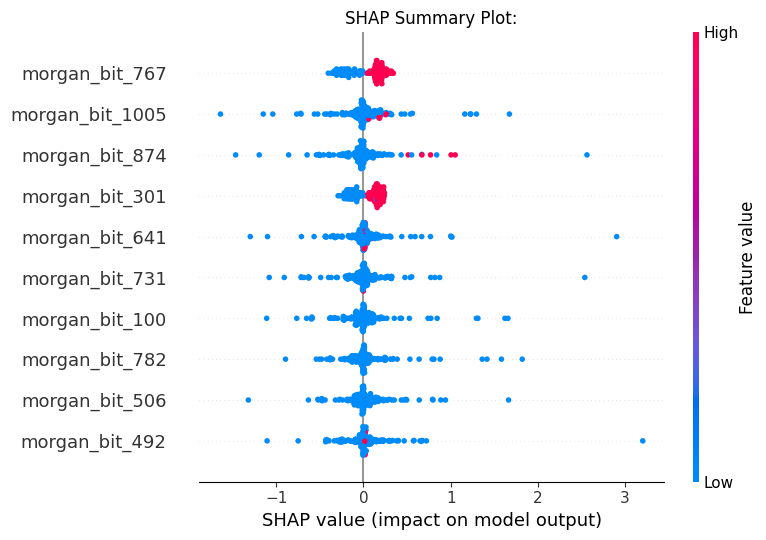
\includegraphics[width=\textwidth, height=0.2\textheight, keepaspectratio]{figures/rf_a_shap.png} % Replace with RF SHAP
        \caption{RF: SHAP Summary}
    \end{subfigure}
    
    \vspace{0.1cm} % Spacer between rows
    
    % ROW 2: CatBoost
    \begin{subfigure}[b]{0.48\textwidth}
        \centering
        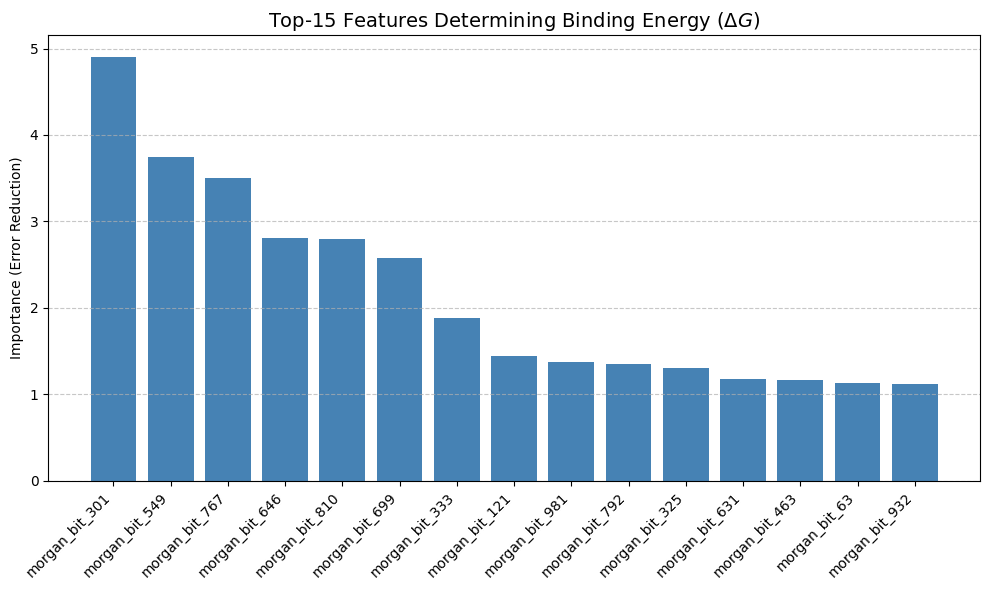
\includegraphics[width=\textwidth, height=0.2\textheight, keepaspectratio]{figures/cb_a_imp.png} % Replace with CatBoost Importance
        \caption{CatBoost: Feature Importance}
    \end{subfigure}
    \hfill
    \begin{subfigure}[b]{0.48\textwidth}
        \centering
        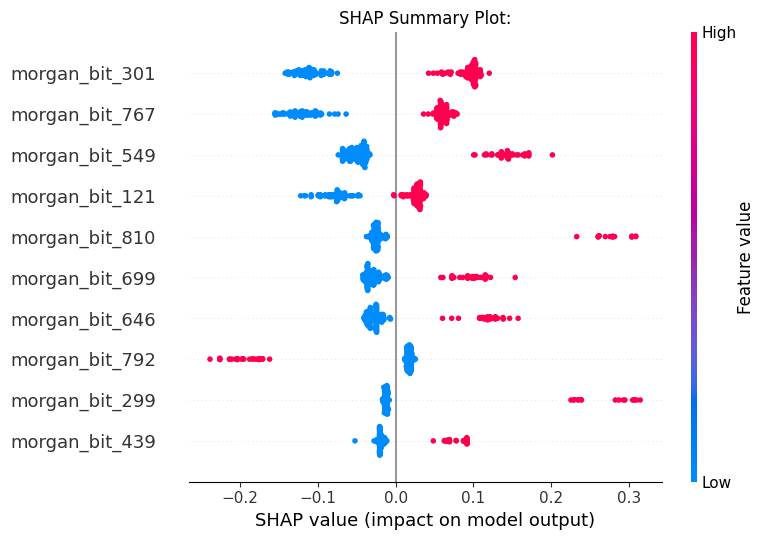
\includegraphics[width=\textwidth, height=0.2\textheight, keepaspectratio]{figures/cb_a_shap.png} % Replace with CatBoost SHAP
        \caption{CatBoost: SHAP Summary}
    \end{subfigure}

    \vspace{0.1cm} % Spacer between rows
    
    % ROW 3: LightGBM
    \begin{subfigure}[b]{0.48\textwidth}
        \centering
        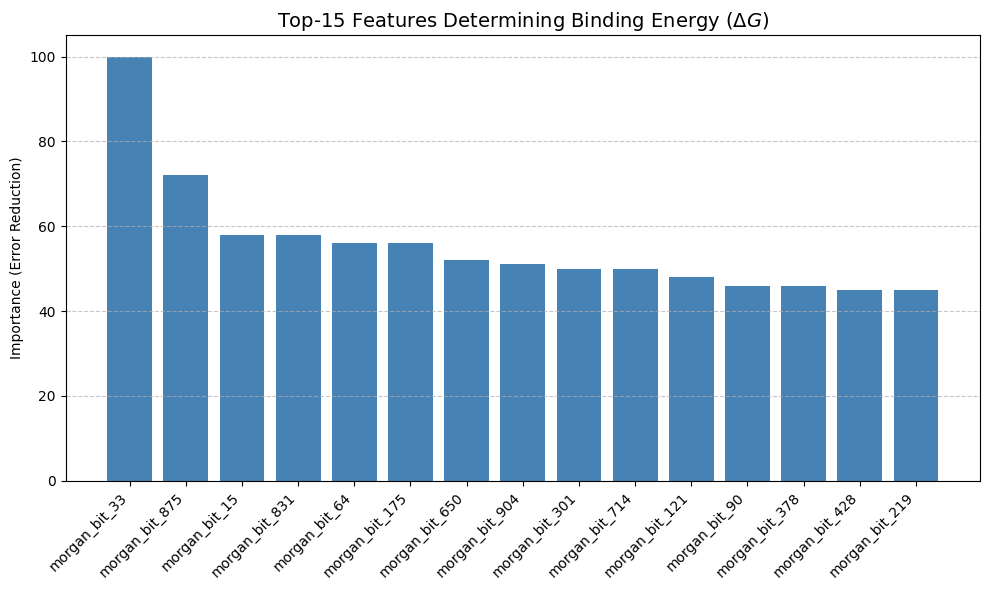
\includegraphics[width=\textwidth, height=0.2\textheight, keepaspectratio]{figures/lgbm_a_imp.png} % Replace with LGBM Importance
        \caption{LGBM: Feature Importance}
    \end{subfigure}
    \hfill
    \begin{subfigure}[b]{0.48\textwidth}
        \centering
        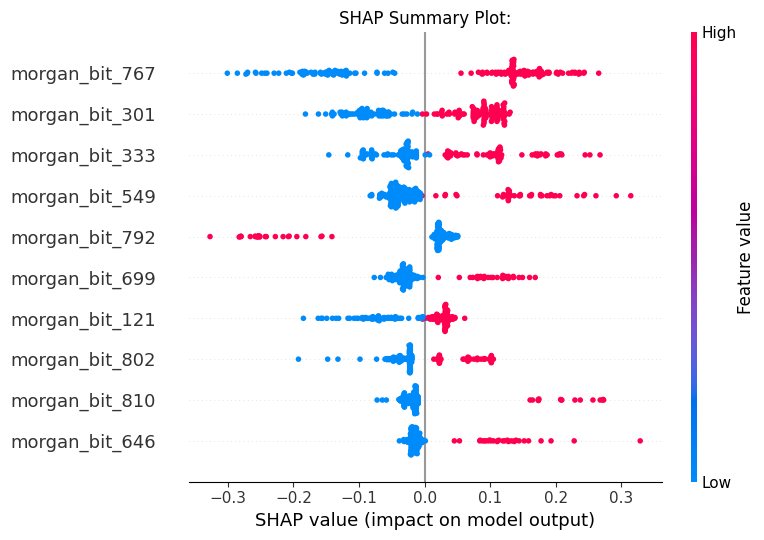
\includegraphics[width=\textwidth, height=0.2\textheight, keepaspectratio]{figures/lgbm_a_shap.png} % Replace with LGBM SHAP
        \caption{LGBM: SHAP Summary}
    \end{subfigure}

    \vspace{0.1cm} % Spacer between rows

    % ROW 4: XGBoost
    \begin{subfigure}[b]{0.48\textwidth}
        \centering
        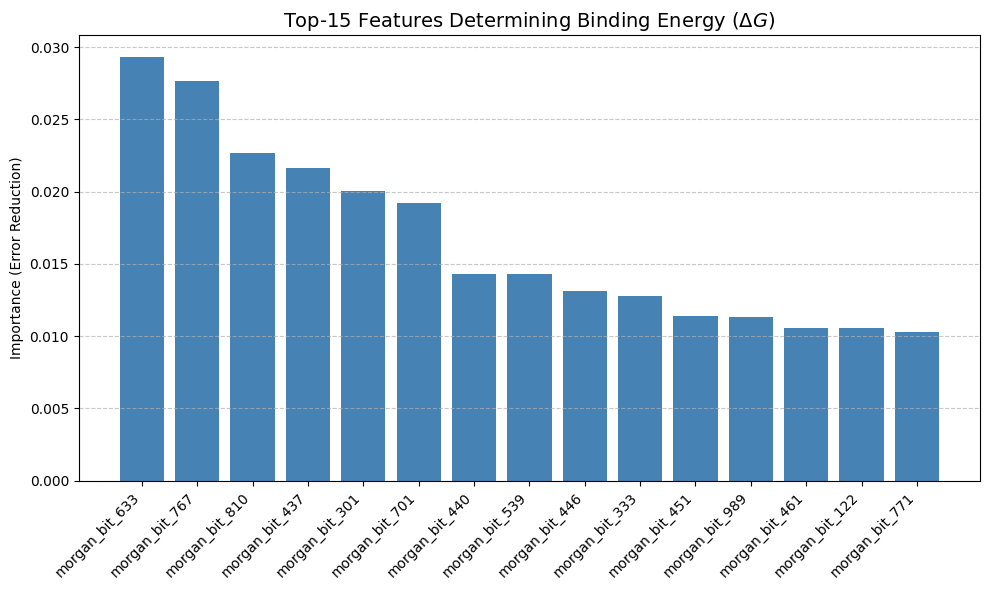
\includegraphics[width=\textwidth, height=0.2\textheight, keepaspectratio]{figures/xgb_a_imp.png} % Replace with XGBoost Importance
        \caption{XGBoost: Feature Importance}
    \end{subfigure}
    \hfill
    \begin{subfigure}[b]{0.48\textwidth}
        \centering
        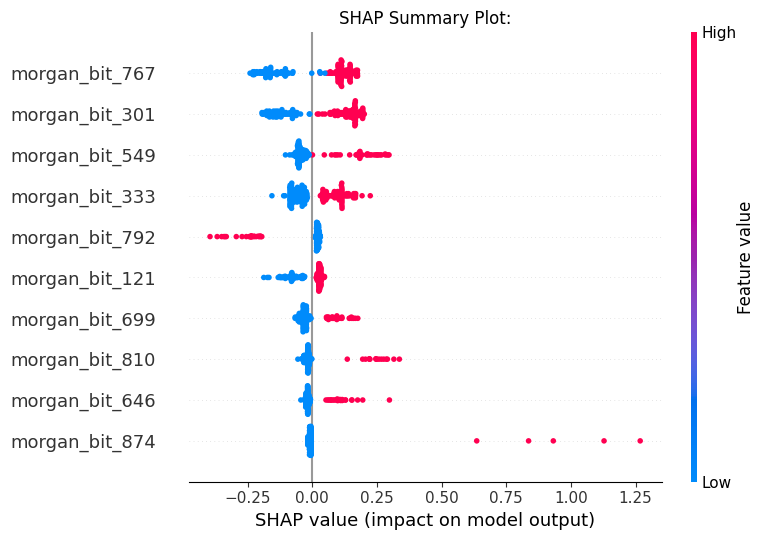
\includegraphics[width=\textwidth, height=0.2\textheight, keepaspectratio]{figures/xgb_a_shap.png} % Replace with XGBoost SHAP
        \caption{XGBoost: SHAP Summary}
    \end{subfigure}

    \caption{Interpretability grid for Experiment A (Morgan Fingerprints Only)}
    \label{fig:expA_grid}
\end{figure}

\begin{figure}[p]
    \centering
    % ROW 1: Random Forest
    \begin{subfigure}[b]{0.48\textwidth}
        \centering
        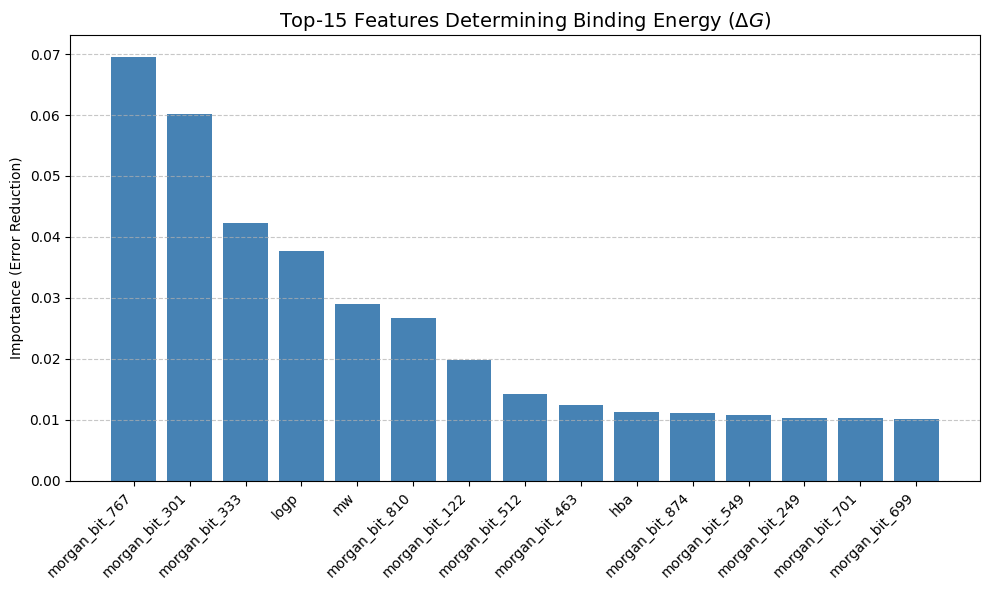
\includegraphics[width=\textwidth, height=0.2\textheight, keepaspectratio]{figures/rf_b_imp.png} % Replace with RF Importance
        \caption{RF: Feature Importance}
    \end{subfigure}
    \hfill
    \begin{subfigure}[b]{0.48\textwidth}
        \centering
        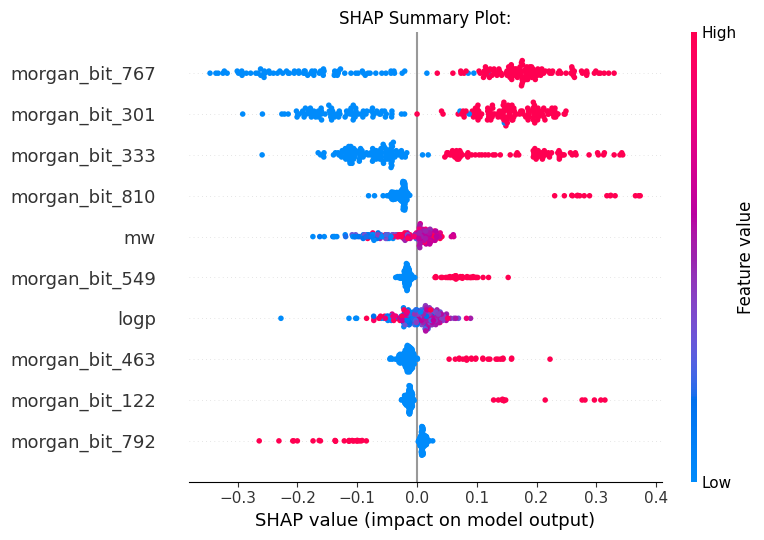
\includegraphics[width=\textwidth, height=0.2\textheight, keepaspectratio]{figures/rf_b_shap.png} % Replace with RF SHAP
        \caption{RF: SHAP Summary}
    \end{subfigure}
    
    \vspace{0.1cm} % Spacer between rows
    
    % ROW 2: CatBoost
    \begin{subfigure}[b]{0.48\textwidth}
        \centering
        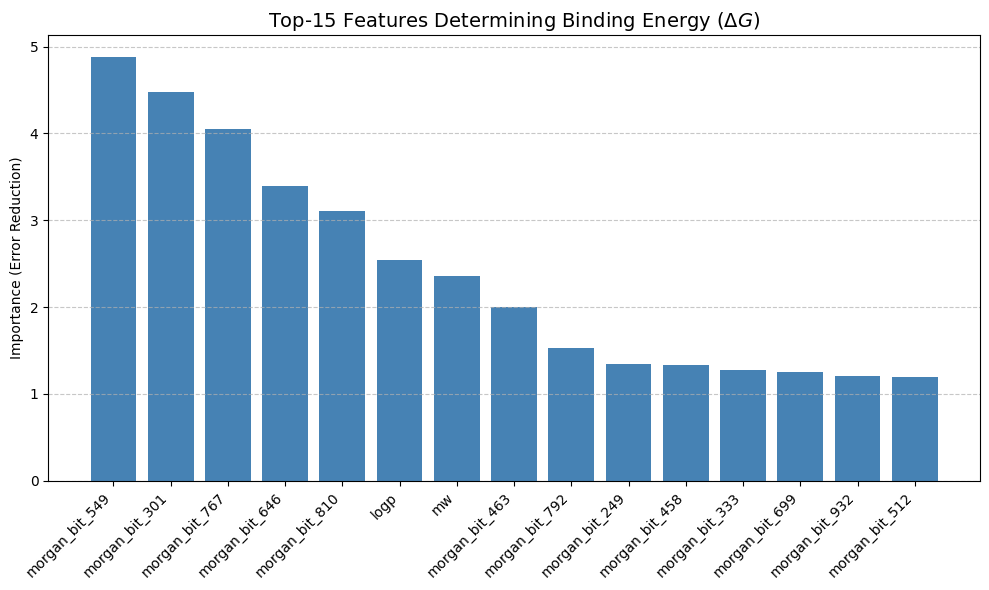
\includegraphics[width=\textwidth, height=0.2\textheight, keepaspectratio]{figures/cb_b_imp.png} % Replace with CatBoost Importance
        \caption{CatBoost: Feature Importance}
    \end{subfigure}
    \hfill
    \begin{subfigure}[b]{0.48\textwidth}
        \centering
        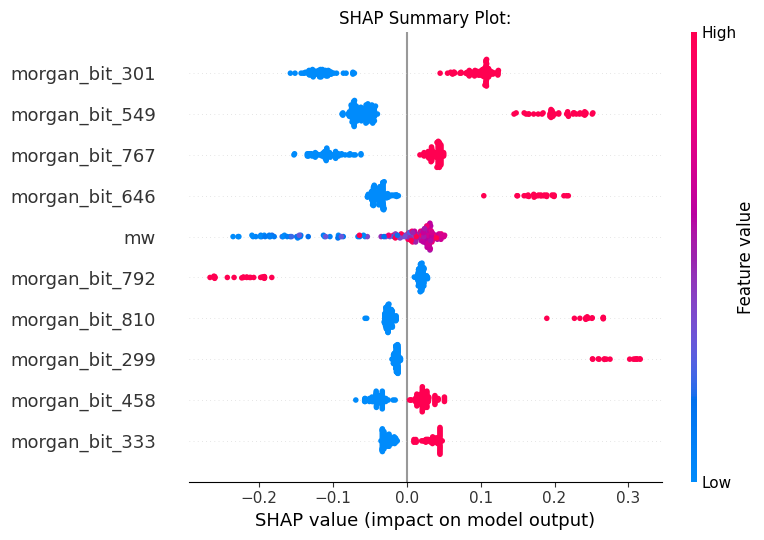
\includegraphics[width=\textwidth, height=0.2\textheight, keepaspectratio]{figures/cb_b_shap.png} % Replace with CatBoost SHAP
        \caption{CatBoost: SHAP Summary}
    \end{subfigure}

    \vspace{0.1cm} % Spacer between rows
    
    % ROW 3: LightGBM
    \begin{subfigure}[b]{0.48\textwidth}
        \centering
        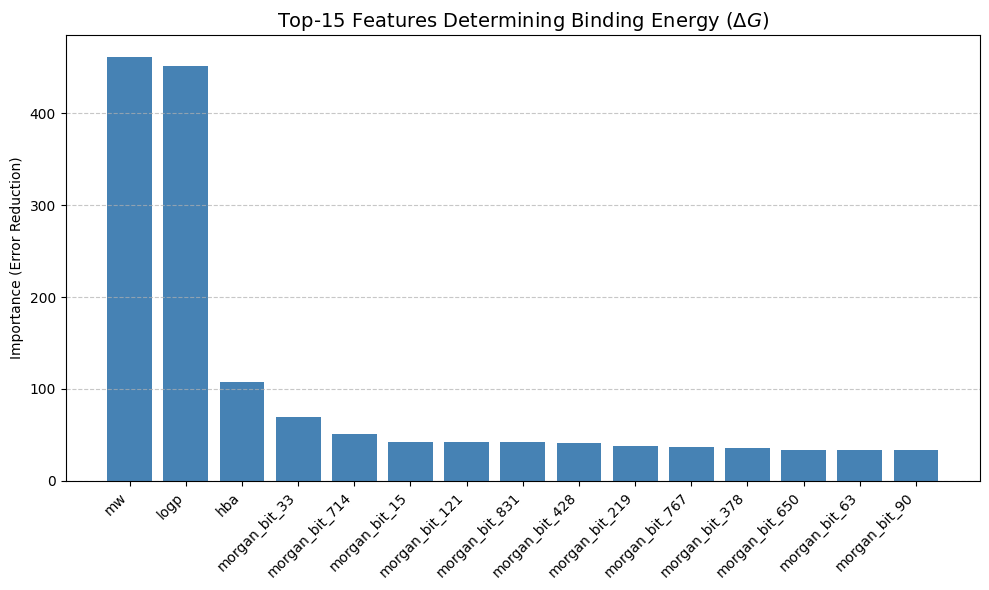
\includegraphics[width=\textwidth, height=0.2\textheight, keepaspectratio]{figures/lgbm_b_imp.png} % Replace with LGBM Importance
        \caption{LGBM: Feature Importance}
    \end{subfigure}
    \hfill
    \begin{subfigure}[b]{0.48\textwidth}
        \centering
        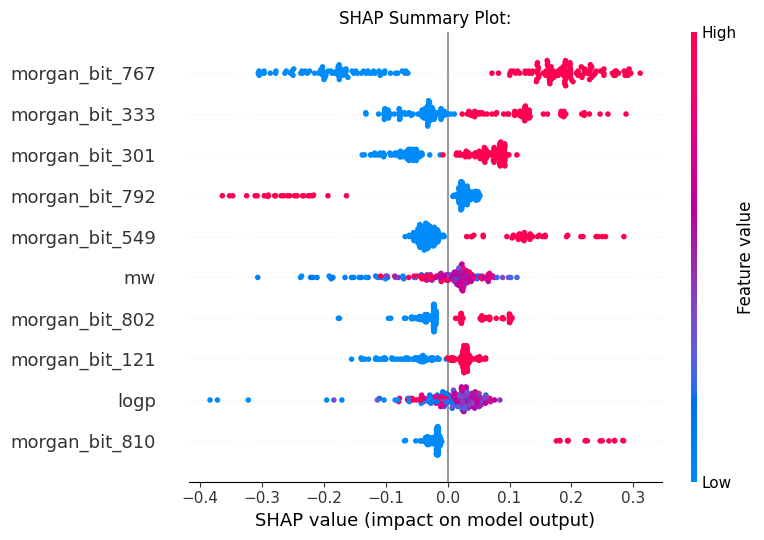
\includegraphics[width=\textwidth, height=0.2\textheight, keepaspectratio]{figures/lgbm_b_shap.png} % Replace with LGBM SHAP
        \caption{LGBM: SHAP Summary}
    \end{subfigure}

    \vspace{0.1cm} % Spacer between rows

    % ROW 4: XGBoost
    \begin{subfigure}[b]{0.48\textwidth}
        \centering
        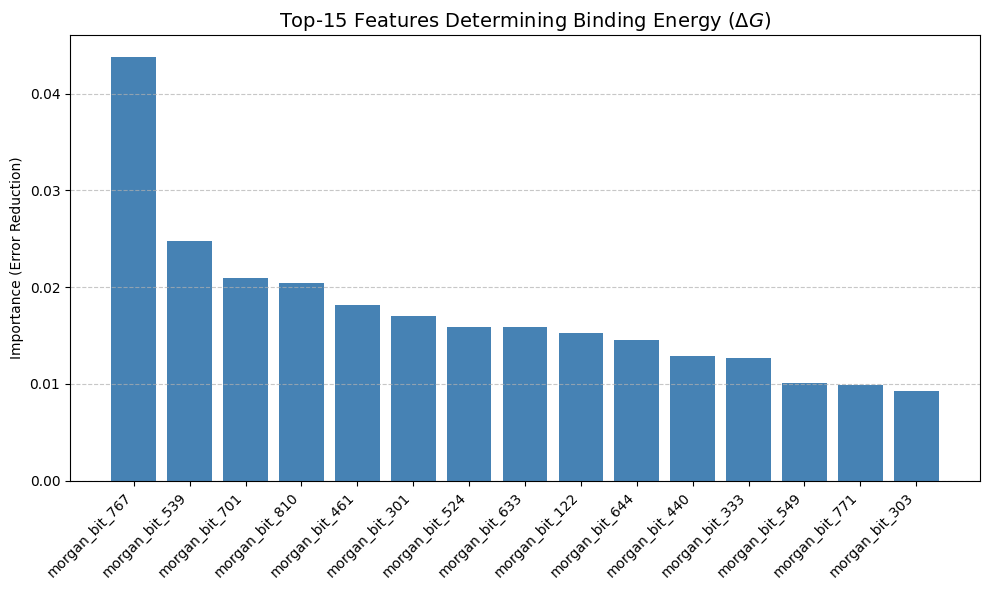
\includegraphics[width=\textwidth, height=0.2\textheight, keepaspectratio]{figures/xgb_b_imp.png} % Replace with XGBoost Importance
        \caption{XGBoost: Feature Importance}
    \end{subfigure}
    \hfill
    \begin{subfigure}[b]{0.48\textwidth}
        \centering
        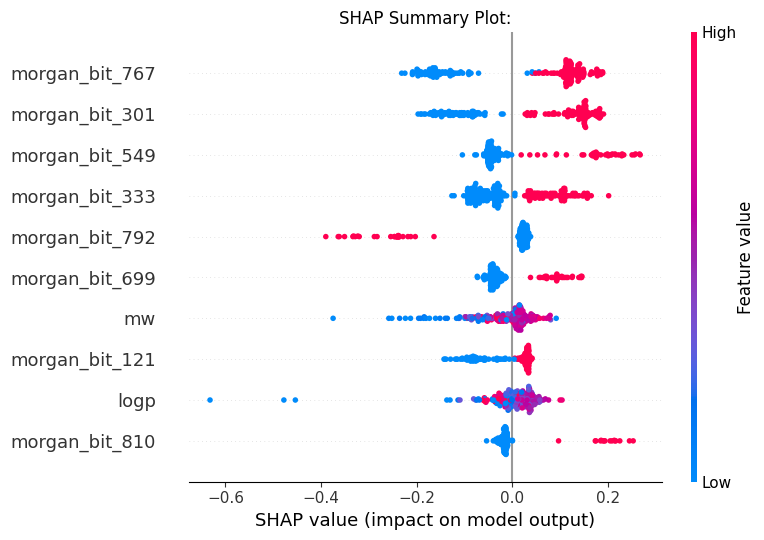
\includegraphics[width=\textwidth, height=0.2\textheight, keepaspectratio]{figures/xgb_b_shap.png} % Replace with XGBoost SHAP
        \caption{XGBoost: SHAP Summary}
    \end{subfigure}

    \caption{Interpretability grid for Experiment B (Morgan Fingerprints + Lipinski's Macro-Prior)}
    \label{fig:expB_grid}
\end{figure}

\begin{figure}[p]
    \centering
    % ROW 1: Random Forest
    \begin{subfigure}[b]{0.48\textwidth}
        \centering
        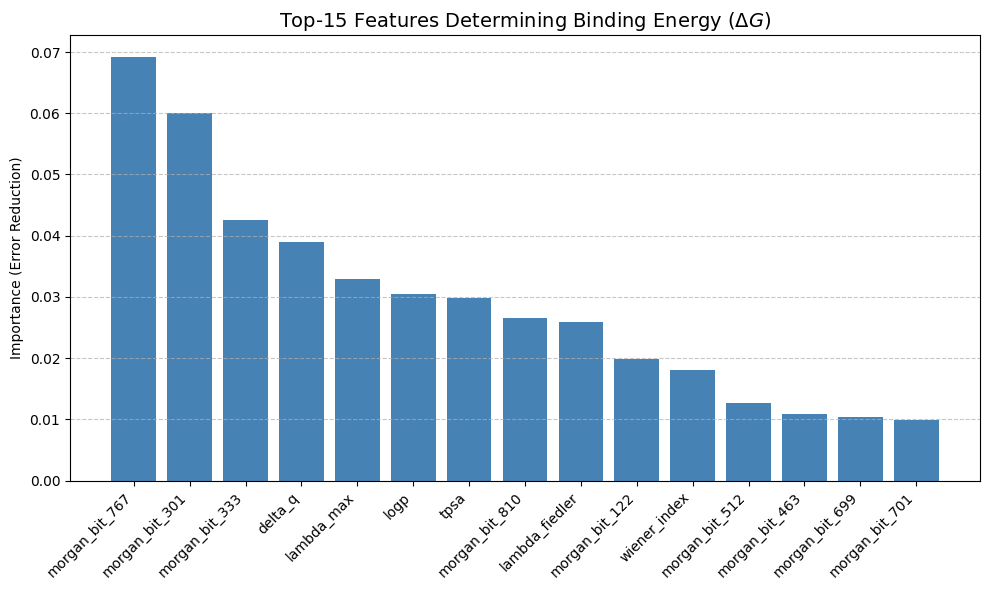
\includegraphics[width=\textwidth, height=0.2\textheight, keepaspectratio]{figures/rf_c_imp.png} % Replace with RF Importance
        \caption{RF: Feature Importance}
    \end{subfigure}
    \hfill
    \begin{subfigure}[b]{0.48\textwidth}
        \centering
        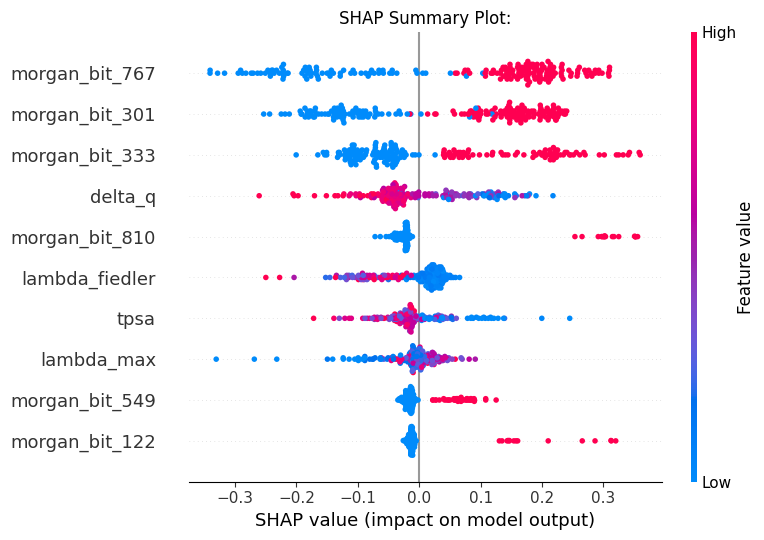
\includegraphics[width=\textwidth, height=0.2\textheight, keepaspectratio]{figures/rf_c_shap.png} % Replace with RF SHAP
        \caption{RF: SHAP Summary}
    \end{subfigure}
    
    \vspace{0.1cm} % Spacer between rows
    
    % ROW 2: CatBoost
    \begin{subfigure}[b]{0.48\textwidth}
        \centering
        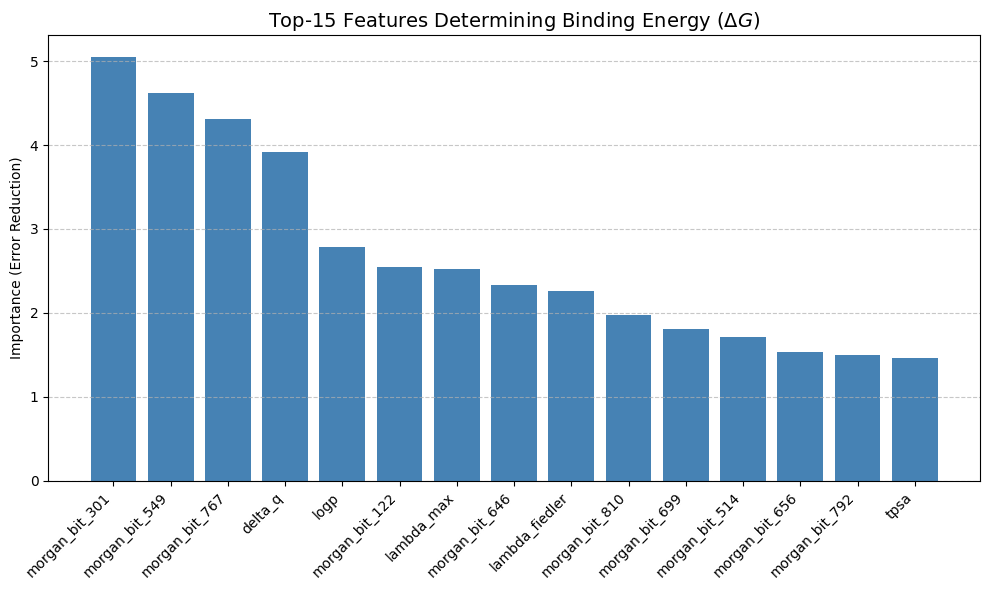
\includegraphics[width=\textwidth, height=0.2\textheight, keepaspectratio]{figures/cb_c_imp.png} % Replace with CatBoost Importance
        \caption{CatBoost: Feature Importance}
    \end{subfigure}
    \hfill
    \begin{subfigure}[b]{0.48\textwidth}
        \centering
        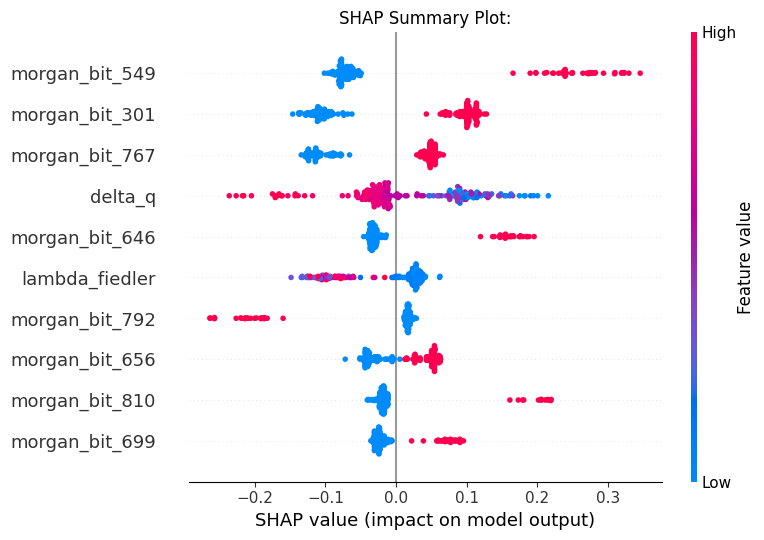
\includegraphics[width=\textwidth, height=0.2\textheight, keepaspectratio]{figures/cb_c_shap.png} % Replace with CatBoost SHAP
        \caption{CatBoost: SHAP Summary}
    \end{subfigure}

    \vspace{0.1cm} % Spacer between rows
    
    % ROW 3: LightGBM
    \begin{subfigure}[b]{0.48\textwidth}
        \centering
        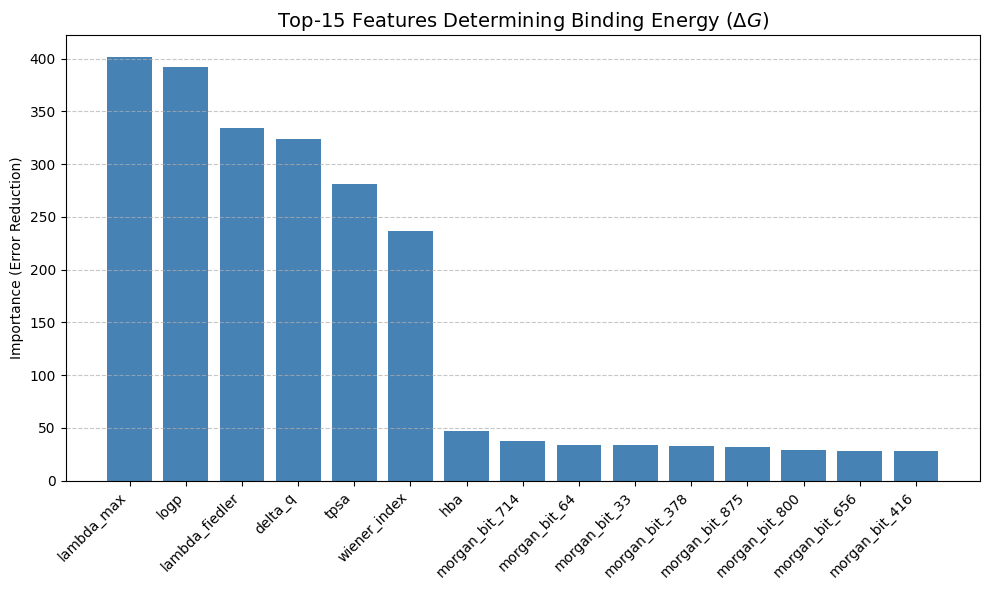
\includegraphics[width=\textwidth, height=0.2\textheight, keepaspectratio]{figures/lgbm_c_imp.png} % Replace with LGBM Importance
        \caption{LGBM: Feature Importance}
    \end{subfigure}
    \hfill
    \begin{subfigure}[b]{0.48\textwidth}
        \centering
        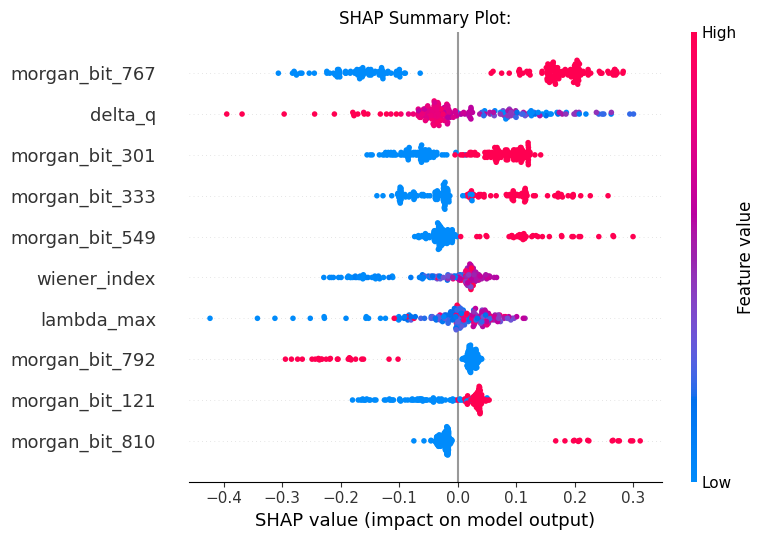
\includegraphics[width=\textwidth, height=0.2\textheight, keepaspectratio]{figures/lgbm_c_shap.png} % Replace with LGBM SHAP
        \caption{LGBM: SHAP Summary}
    \end{subfigure}

    \vspace{0.1cm} % Spacer between rows

    % ROW 4: XGBoost
    \begin{subfigure}[b]{0.48\textwidth}
        \centering
        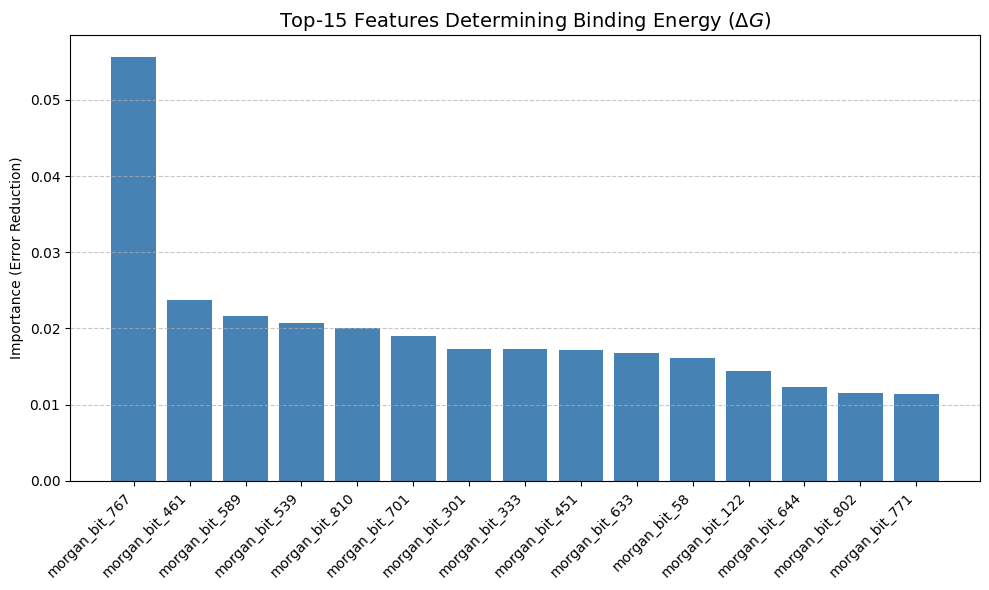
\includegraphics[width=\textwidth, height=0.2\textheight, keepaspectratio]{figures/xgb_c_imp.png} % Replace with XGBoost Importance
        \caption{XGBoost: Feature Importance}
    \end{subfigure}
    \hfill
    \begin{subfigure}[b]{0.48\textwidth}
        \centering
        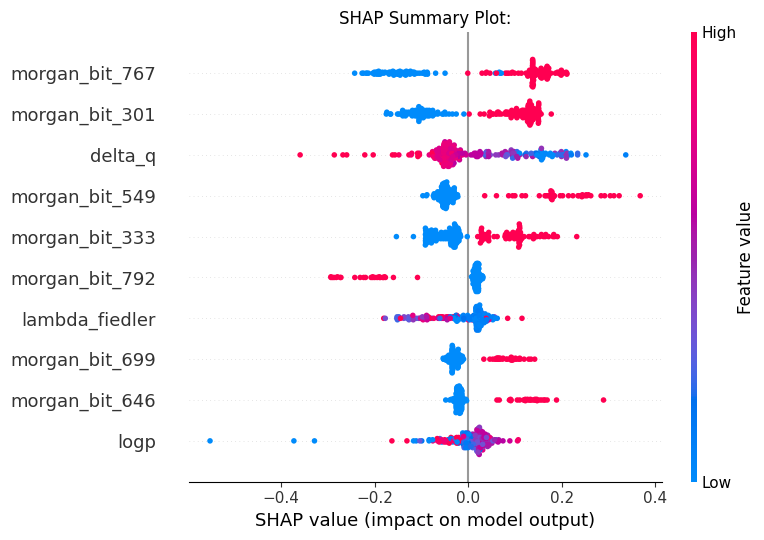
\includegraphics[width=\textwidth, height=0.2\textheight, keepaspectratio]{figures/xgb_c_shap.png} % Replace with XGBoost SHAP
        \caption{XGBoost: SHAP Summary}
    \end{subfigure}

    \caption{Interpretability grid for Experiment C (Morgan Fingerprints + Lipinski's Macro-Prior + 2D Spectral Physics)}
    \label{fig:expC_grid}
\end{figure}

\begin{figure}[p]
    \centering
    % ROW 1: Random Forest
    \begin{subfigure}[b]{0.48\textwidth}
        \centering
        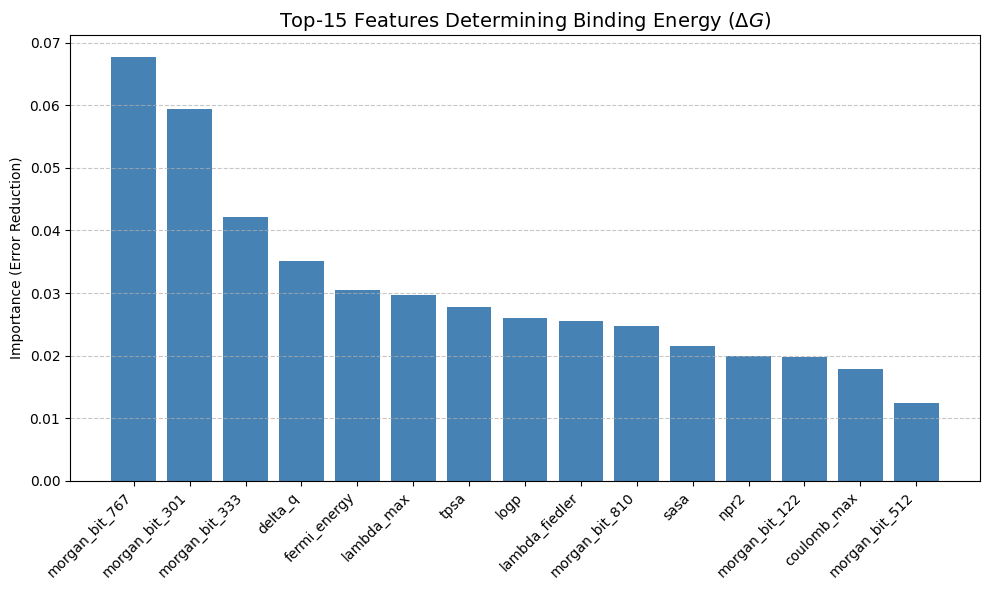
\includegraphics[width=\textwidth, height=0.2\textheight, keepaspectratio]{figures/rf_d_imp.png} % Replace with RF Importance
        \caption{RF: Feature Importance}
    \end{subfigure}
    \hfill
    \begin{subfigure}[b]{0.48\textwidth}
        \centering
        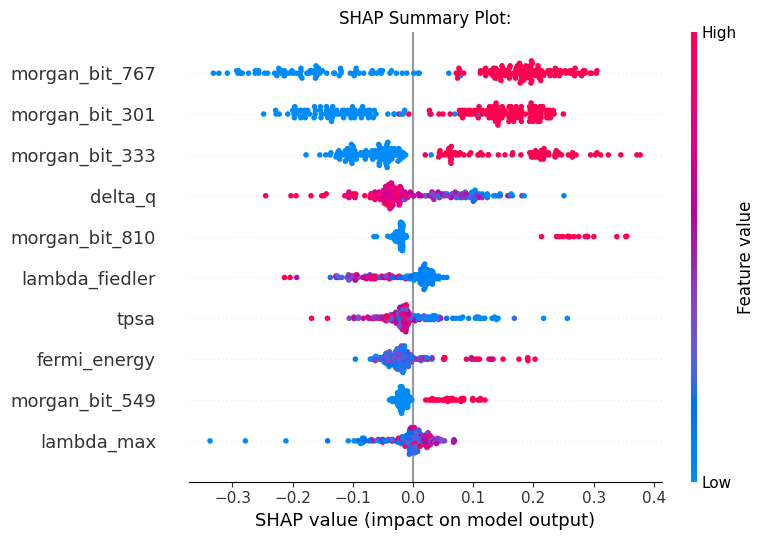
\includegraphics[width=\textwidth, height=0.2\textheight, keepaspectratio]{figures/rf_d_shap.png} % Replace with RF SHAP
        \caption{RF: SHAP Summary}
    \end{subfigure}
    
    \vspace{0.1cm} % Spacer between rows
    
    % ROW 2: CatBoost
    \begin{subfigure}[b]{0.48\textwidth}
        \centering
        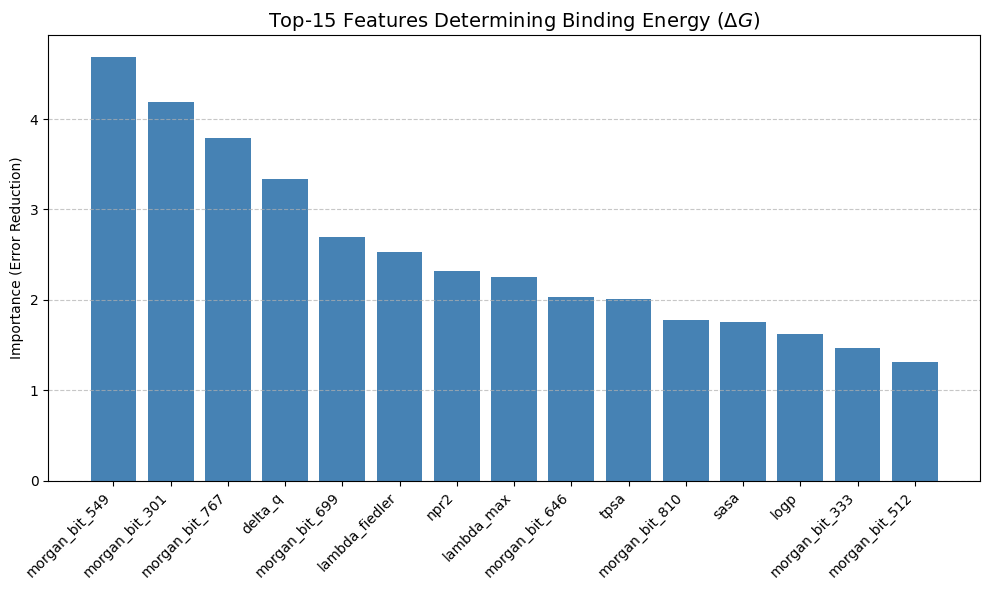
\includegraphics[width=\textwidth, height=0.2\textheight, keepaspectratio]{figures/cb_d_imp.png} % Replace with CatBoost Importance
        \caption{CatBoost: Feature Importance}
    \end{subfigure}
    \hfill
    \begin{subfigure}[b]{0.48\textwidth}
        \centering
        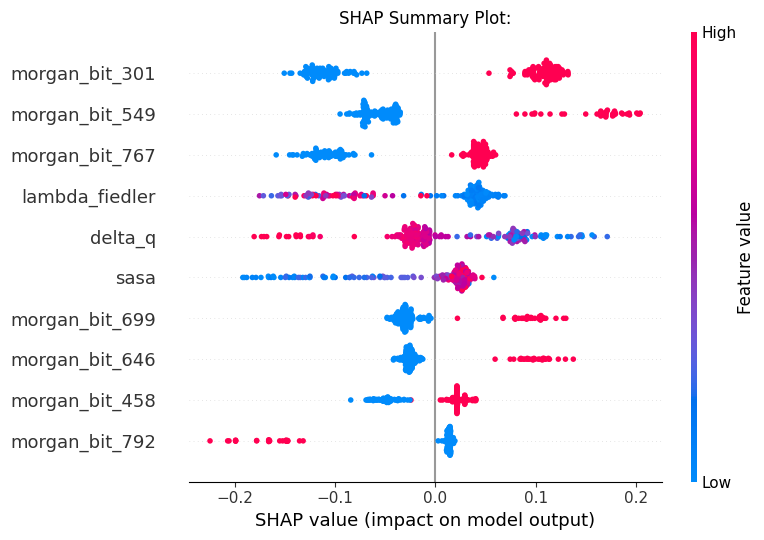
\includegraphics[width=\textwidth, height=0.2\textheight, keepaspectratio]{figures/cb_d_shap.png} % Replace with CatBoost SHAP
        \caption{CatBoost: SHAP Summary}
    \end{subfigure}

    \vspace{0.1cm} % Spacer between rows
    
    % ROW 3: LightGBM
    \begin{subfigure}[b]{0.48\textwidth}
        \centering
        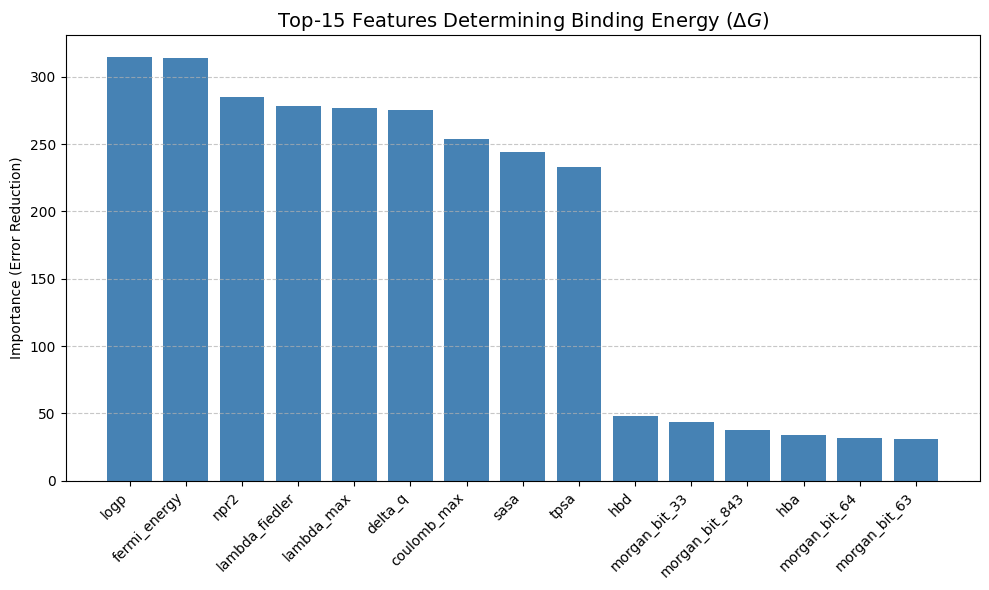
\includegraphics[width=\textwidth, height=0.2\textheight, keepaspectratio]{figures/lgbm_d_imp.png} % Replace with LGBM Importance
        \caption{LGBM: Feature Importance}
    \end{subfigure}
    \hfill
    \begin{subfigure}[b]{0.48\textwidth}
        \centering
        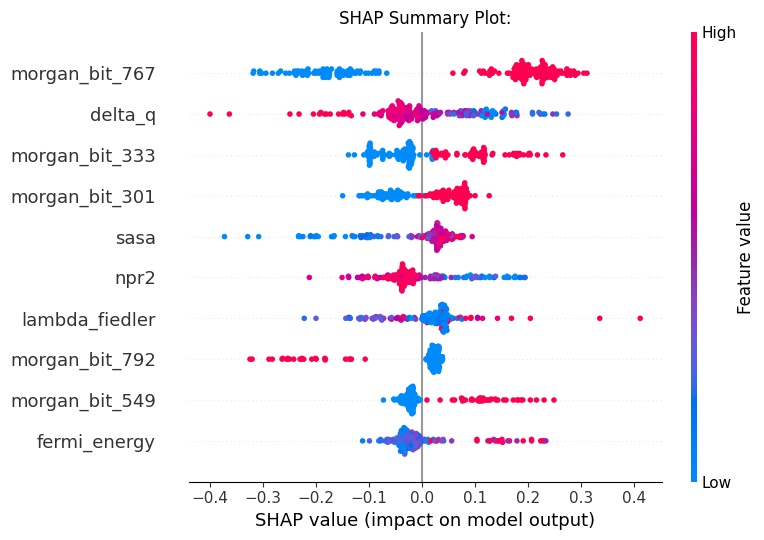
\includegraphics[width=\textwidth, height=0.2\textheight, keepaspectratio]{figures/lgbm_d_shap.png} % Replace with LGBM SHAP
        \caption{LGBM: SHAP Summary}
    \end{subfigure}

    \vspace{0.1cm} % Spacer between rows

    % ROW 4: XGBoost
    \begin{subfigure}[b]{0.48\textwidth}
        \centering
        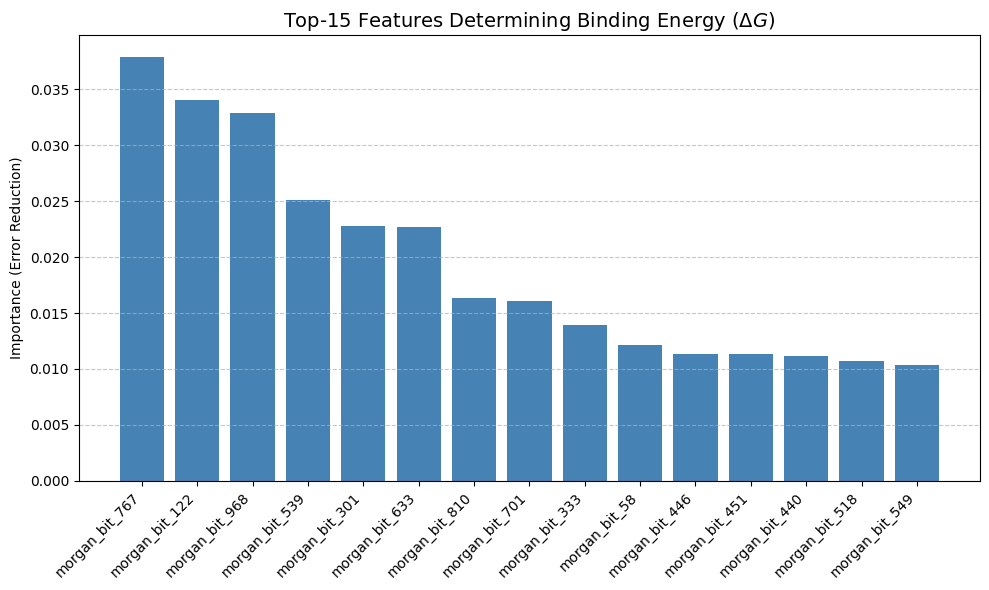
\includegraphics[width=\textwidth, height=0.2\textheight, keepaspectratio]{figures/xgb_d_imp.png} % Replace with XGBoost Importance
        \caption{XGBoost: Feature Importance}
    \end{subfigure}
    \hfill
    \begin{subfigure}[b]{0.48\textwidth}
        \centering
        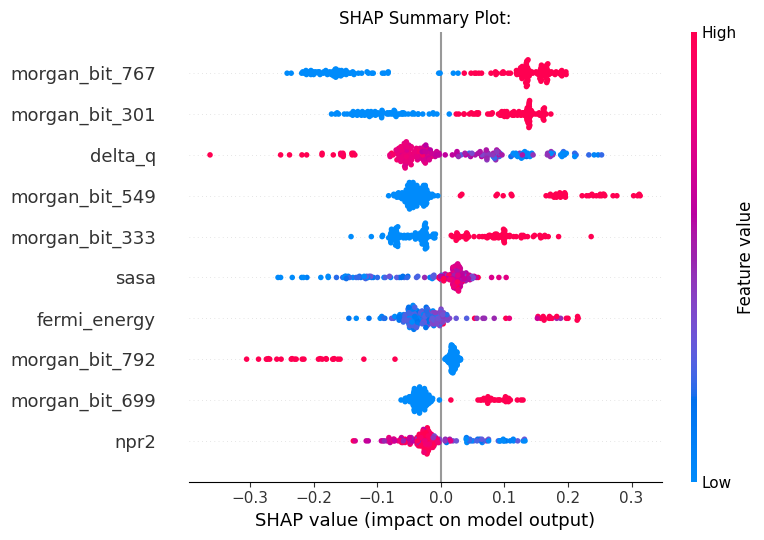
\includegraphics[width=\textwidth, height=0.2\textheight, keepaspectratio]{figures/xgb_d_shap.png} % Replace with XGBoost SHAP
        \caption{XGBoost: SHAP Summary}
    \end{subfigure}

    \caption{Interpretability grid for Experiment D (Morgan Fingerprints + Lipinski's Macro-Prior + 2D Spectral Physics + 3D Quantum/Spatial Fields)}
    \label{fig:expD_grid}
\end{figure}

\begin{figure}[p]
    \centering
    % ROW 1: Random Forest
    \begin{subfigure}[b]{0.48\textwidth}
        \centering
        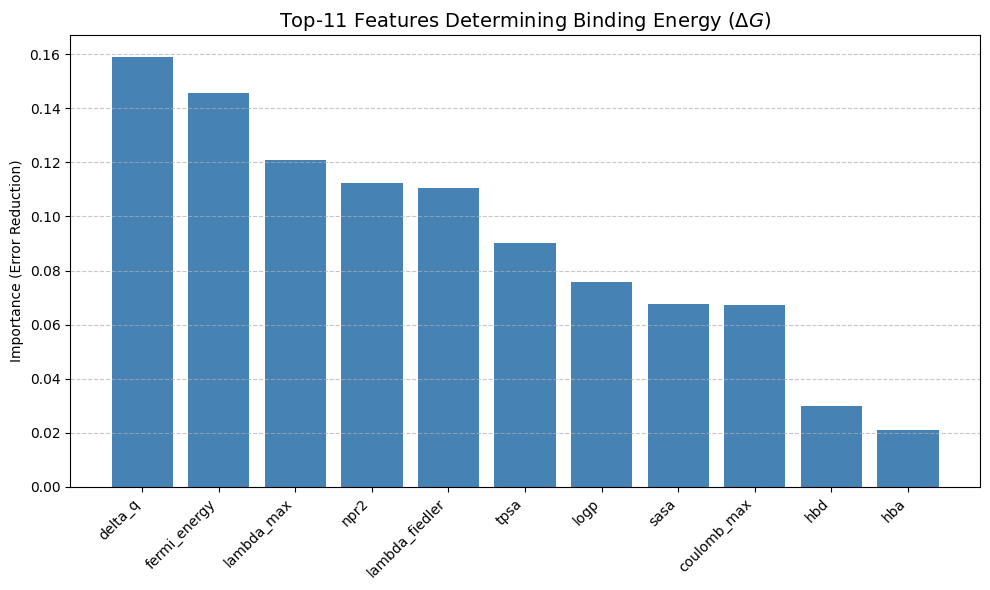
\includegraphics[width=\textwidth, height=0.2\textheight, keepaspectratio]{figures/rf_e_imp.png} % Replace with RF Importance
        \caption{RF: Feature Importance}
    \end{subfigure}
    \hfill
    \begin{subfigure}[b]{0.48\textwidth}
        \centering
        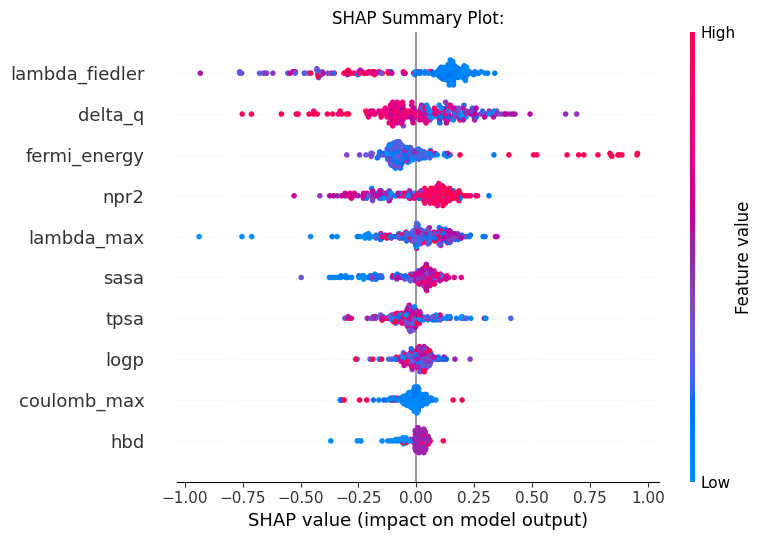
\includegraphics[width=\textwidth, height=0.2\textheight, keepaspectratio]{figures/rf_e_shap.png} % Replace with RF SHAP
        \caption{RF: SHAP Summary}
    \end{subfigure}
    
    \vspace{0.1cm} % Spacer between rows
    
    % ROW 2: CatBoost
    \begin{subfigure}[b]{0.48\textwidth}
        \centering
        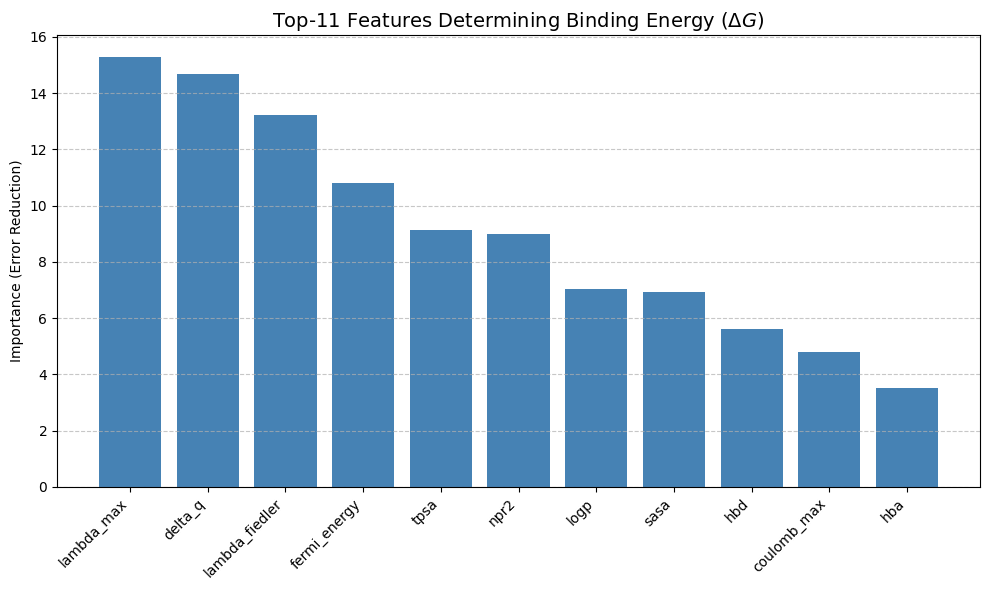
\includegraphics[width=\textwidth, height=0.2\textheight, keepaspectratio]{figures/cb_e_imp.png} % Replace with CatBoost Importance
        \caption{CatBoost: Feature Importance}
    \end{subfigure}
    \hfill
    \begin{subfigure}[b]{0.48\textwidth}
        \centering
        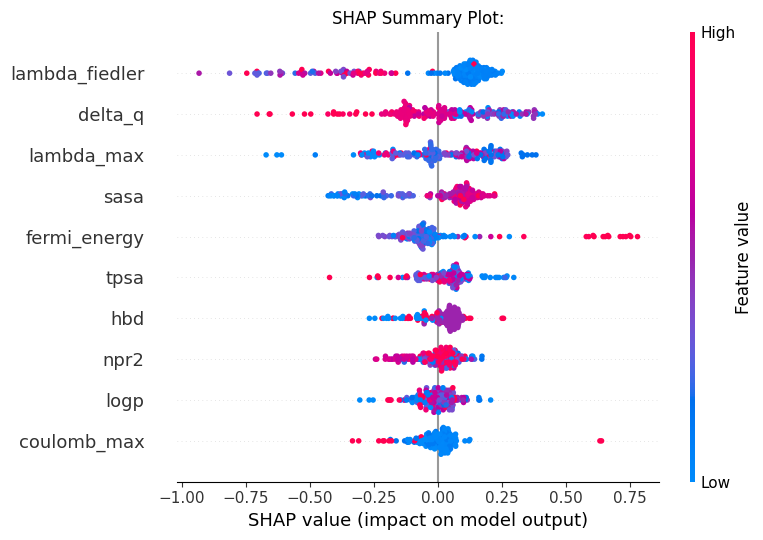
\includegraphics[width=\textwidth, height=0.2\textheight, keepaspectratio]{figures/cb_e_shap.png} % Replace with CatBoost SHAP
        \caption{CatBoost: SHAP Summary}
    \end{subfigure}

    \vspace{0.1cm} % Spacer between rows
    
    % ROW 3: LightGBM
    \begin{subfigure}[b]{0.48\textwidth}
        \centering
        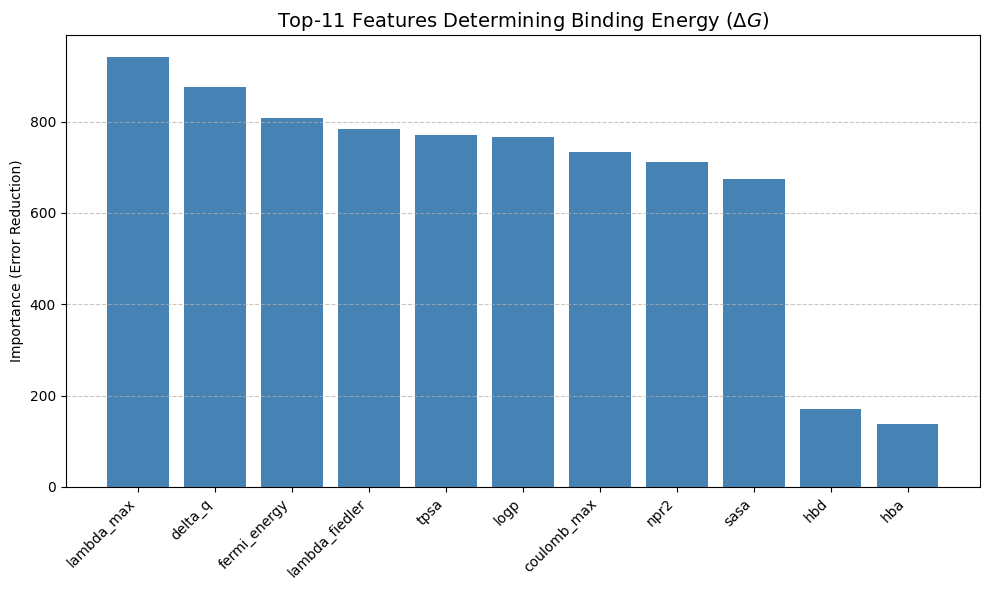
\includegraphics[width=\textwidth, height=0.2\textheight, keepaspectratio]{figures/lgbm_e_imp.png} % Replace with LGBM Importance
        \caption{LGBM: Feature Importance}
    \end{subfigure}
    \hfill
    \begin{subfigure}[b]{0.48\textwidth}
        \centering
        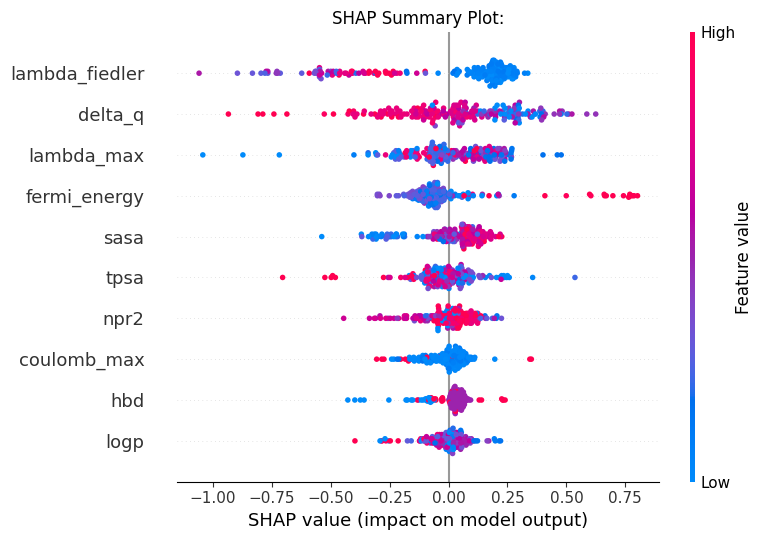
\includegraphics[width=\textwidth, height=0.2\textheight, keepaspectratio]{figures/lgbm_e_shap.png} % Replace with LGBM SHAP
        \caption{LGBM: SHAP Summary}
    \end{subfigure}

    \vspace{0.1cm} % Spacer between rows

    % ROW 4: XGBoost
    \begin{subfigure}[b]{0.48\textwidth}
        \centering
        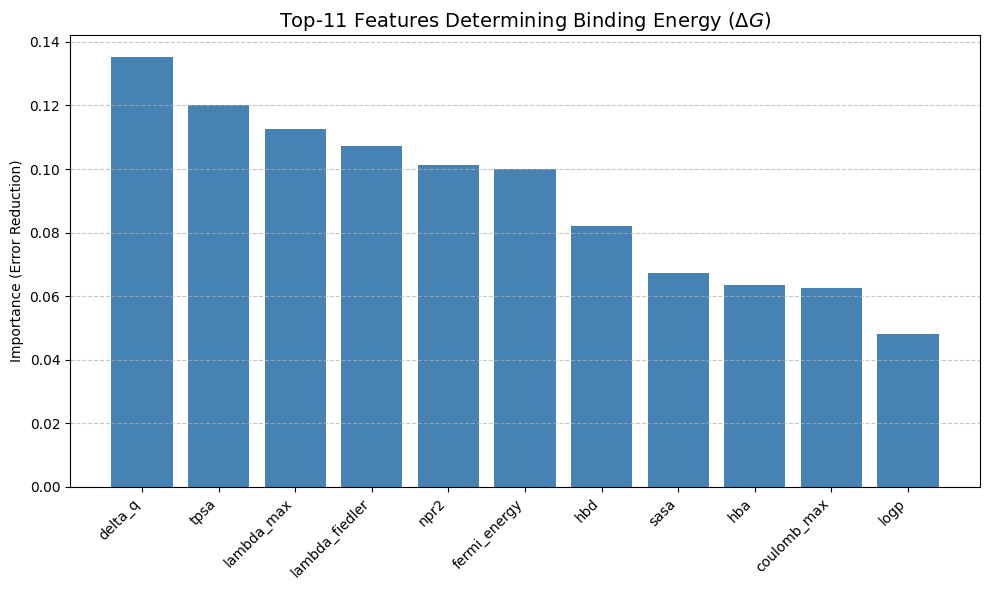
\includegraphics[width=\textwidth, height=0.2\textheight, keepaspectratio]{figures/xgb_e_imp.png} % Replace with XGBoost Importance
        \caption{XGBoost: Feature Importance}
    \end{subfigure}
    \hfill
    \begin{subfigure}[b]{0.48\textwidth}
        \centering
        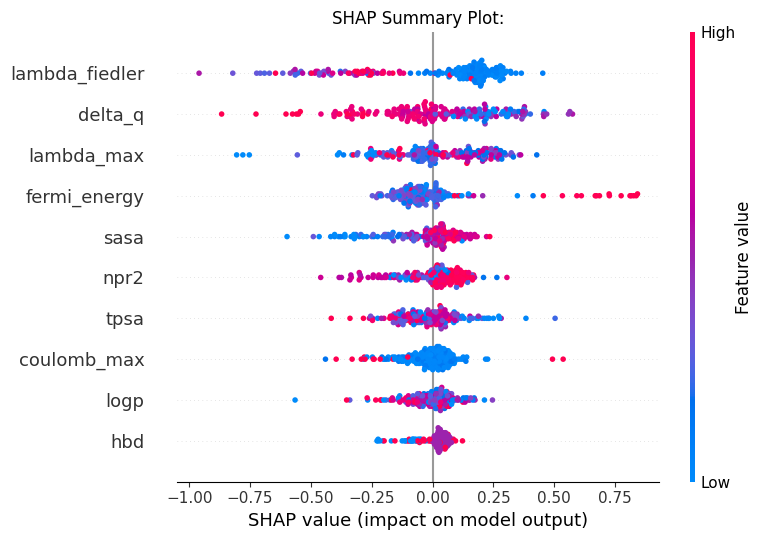
\includegraphics[width=\textwidth, height=0.2\textheight, keepaspectratio]{figures/xgb_e_shap.png} % Replace with XGBoost SHAP
        \caption{XGBoost: SHAP Summary}
    \end{subfigure}

    \caption{Interpretability grid for Experiment E (Pure Physics: Macroscopic Thermodynamics + 2D Spectral Physics + 3D Quantum/Spatial Fields)}
    \label{fig:expE_grid}
\end{figure}

\subsection*{3.5. Discussion and Analytical Insights}

The experimental results (Table \ref{tab:results}) and SHAP analyses (Figures \ref{fig:expA_grid}-\ref{fig:expE_grid}) reveal a profound narrative
about how machine learning models interpret chemical space:

\textbf{3.5.1. The Dominance of Topological Anchors (Experiments A \& B):}

Across experiments containing Morgan fingerprints, tree-based models consistently relied on a highly sparse subset of topological bits to drive
predictions. As illustrated in Figure \ref{fig:morgan_bits}, visual inspection of these top-ranked substructures across all architectures reveals
that they represent a functionally diverse set of pharmacophores rather than arbitrary structural noise. 

These dominant bits fundamentally differ in their intrinsic properties: from rigid aromatic constraints to flexible aliphatic configurations,
ensuring different degrees of conformational freedom. Furthermore, they encompass a broad spectrum of interaction potentials, including varying
hydrogen-bond donor and acceptor capacities, structural motifs capable of salt-bridge formation, and distinct steric profiles required for
penetrating specific sub-pockets of the receptor. 

\begin{figure}[H]
    \centering
    \begin{subfigure}[b]{0.24\textwidth}
        \centering
        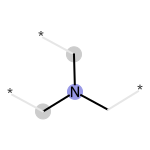
\includegraphics[width=\textwidth]{figures/bit_767.png}
        \caption{Bit 767}
    \end{subfigure}
    \hfill
    \begin{subfigure}[b]{0.24\textwidth}
        \centering
        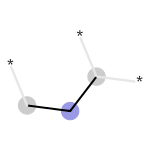
\includegraphics[width=\textwidth]{figures/bit_301.png}
        \caption{Bit 301}
    \end{subfigure}
    \hfill
    \begin{subfigure}[b]{0.24\textwidth}
        \centering
        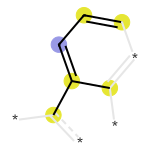
\includegraphics[width=\textwidth]{figures/bit_549.png}
        \caption{Bit 549}
    \end{subfigure}
    \hfill
    \begin{subfigure}[b]{0.24\textwidth}
        \centering
        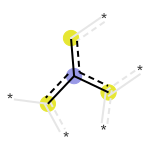
\includegraphics[width=\textwidth]{figures/bit_333.png}
        \caption{Bit 333}
    \end{subfigure}
    \caption{\textbf{Dominant Topological Anchors:} Visual representation of the most impactful Morgan fingerprint bits consistently identified
    by tree-based estimators. The selected substructures demonstrate the functional diversity prioritized by the models, encompassing a range
    of structural flexibilities, spatial configurations, and distinct physicochemical properties required for optimal receptor-ligand interactions.}

    \label{fig:morgan_bits}
\end{figure}

\textbf{3.5.2. The Pure Physics Paradigm (Experiment E):}
The most critical finding emerges from Experiment E, where we forcefully removed all 1024 Morgan bits and Lipinski heuristics, forcing
the models to predict $\Delta G$ using only the 11-dimensional orthogonal basis of continuous fields. While the performance of Experiment E
is predictably lower than the topological experiments, it is remarkable that the models can still achieve a respectable result using only
fundamental physical descriptors. This suggests that the underlying thermodynamic and quantum mechanical properties of the molecules do contain
significant predictive signal for binding affinity, even in the absence of explicit topological fingerprints.

The SHAP analyses for Experiment E reveal that the models are primarily leveraging global graph connectivity ($\lambda_{max}$, $\lambda_{fiedler}$)
to establish the baseline affinity. The predictions are then fine-tuned using precise spatial and electrostatic fields (\texttt{delta\_q},
and \texttt{fermi\_energy}). This confirms that while tree ensembles excel at discrete pattern matching (as seen with Morgan fingerprints),
they are fully capable of approximating the underlying continuous physics when topological "shortcuts" are explicitly removed.

\end{document}
